% Options for packages loaded elsewhere
\PassOptionsToPackage{unicode}{hyperref}
\PassOptionsToPackage{hyphens}{url}
%
\documentclass[
]{article}
\title{Lab sheet 3: R Programming}
\author{}
\date{\vspace{-2.5em}}

\usepackage{amsmath,amssymb}
\usepackage{lmodern}
\usepackage{iftex}
\ifPDFTeX
  \usepackage[T1]{fontenc}
  \usepackage[utf8]{inputenc}
  \usepackage{textcomp} % provide euro and other symbols
\else % if luatex or xetex
  \usepackage{unicode-math}
  \defaultfontfeatures{Scale=MatchLowercase}
  \defaultfontfeatures[\rmfamily]{Ligatures=TeX,Scale=1}
\fi
% Use upquote if available, for straight quotes in verbatim environments
\IfFileExists{upquote.sty}{\usepackage{upquote}}{}
\IfFileExists{microtype.sty}{% use microtype if available
  \usepackage[]{microtype}
  \UseMicrotypeSet[protrusion]{basicmath} % disable protrusion for tt fonts
}{}
\makeatletter
\@ifundefined{KOMAClassName}{% if non-KOMA class
  \IfFileExists{parskip.sty}{%
    \usepackage{parskip}
  }{% else
    \setlength{\parindent}{0pt}
    \setlength{\parskip}{6pt plus 2pt minus 1pt}}
}{% if KOMA class
  \KOMAoptions{parskip=half}}
\makeatother
\usepackage{xcolor}
\IfFileExists{xurl.sty}{\usepackage{xurl}}{} % add URL line breaks if available
\IfFileExists{bookmark.sty}{\usepackage{bookmark}}{\usepackage{hyperref}}
\hypersetup{
  pdftitle={Lab sheet 3: R Programming},
  hidelinks,
  pdfcreator={LaTeX via pandoc}}
\urlstyle{same} % disable monospaced font for URLs
\usepackage[margin=1in]{geometry}
\usepackage{color}
\usepackage{fancyvrb}
\newcommand{\VerbBar}{|}
\newcommand{\VERB}{\Verb[commandchars=\\\{\}]}
\DefineVerbatimEnvironment{Highlighting}{Verbatim}{commandchars=\\\{\}}
% Add ',fontsize=\small' for more characters per line
\usepackage{framed}
\definecolor{shadecolor}{RGB}{248,248,248}
\newenvironment{Shaded}{\begin{snugshade}}{\end{snugshade}}
\newcommand{\AlertTok}[1]{\textcolor[rgb]{0.94,0.16,0.16}{#1}}
\newcommand{\AnnotationTok}[1]{\textcolor[rgb]{0.56,0.35,0.01}{\textbf{\textit{#1}}}}
\newcommand{\AttributeTok}[1]{\textcolor[rgb]{0.77,0.63,0.00}{#1}}
\newcommand{\BaseNTok}[1]{\textcolor[rgb]{0.00,0.00,0.81}{#1}}
\newcommand{\BuiltInTok}[1]{#1}
\newcommand{\CharTok}[1]{\textcolor[rgb]{0.31,0.60,0.02}{#1}}
\newcommand{\CommentTok}[1]{\textcolor[rgb]{0.56,0.35,0.01}{\textit{#1}}}
\newcommand{\CommentVarTok}[1]{\textcolor[rgb]{0.56,0.35,0.01}{\textbf{\textit{#1}}}}
\newcommand{\ConstantTok}[1]{\textcolor[rgb]{0.00,0.00,0.00}{#1}}
\newcommand{\ControlFlowTok}[1]{\textcolor[rgb]{0.13,0.29,0.53}{\textbf{#1}}}
\newcommand{\DataTypeTok}[1]{\textcolor[rgb]{0.13,0.29,0.53}{#1}}
\newcommand{\DecValTok}[1]{\textcolor[rgb]{0.00,0.00,0.81}{#1}}
\newcommand{\DocumentationTok}[1]{\textcolor[rgb]{0.56,0.35,0.01}{\textbf{\textit{#1}}}}
\newcommand{\ErrorTok}[1]{\textcolor[rgb]{0.64,0.00,0.00}{\textbf{#1}}}
\newcommand{\ExtensionTok}[1]{#1}
\newcommand{\FloatTok}[1]{\textcolor[rgb]{0.00,0.00,0.81}{#1}}
\newcommand{\FunctionTok}[1]{\textcolor[rgb]{0.00,0.00,0.00}{#1}}
\newcommand{\ImportTok}[1]{#1}
\newcommand{\InformationTok}[1]{\textcolor[rgb]{0.56,0.35,0.01}{\textbf{\textit{#1}}}}
\newcommand{\KeywordTok}[1]{\textcolor[rgb]{0.13,0.29,0.53}{\textbf{#1}}}
\newcommand{\NormalTok}[1]{#1}
\newcommand{\OperatorTok}[1]{\textcolor[rgb]{0.81,0.36,0.00}{\textbf{#1}}}
\newcommand{\OtherTok}[1]{\textcolor[rgb]{0.56,0.35,0.01}{#1}}
\newcommand{\PreprocessorTok}[1]{\textcolor[rgb]{0.56,0.35,0.01}{\textit{#1}}}
\newcommand{\RegionMarkerTok}[1]{#1}
\newcommand{\SpecialCharTok}[1]{\textcolor[rgb]{0.00,0.00,0.00}{#1}}
\newcommand{\SpecialStringTok}[1]{\textcolor[rgb]{0.31,0.60,0.02}{#1}}
\newcommand{\StringTok}[1]{\textcolor[rgb]{0.31,0.60,0.02}{#1}}
\newcommand{\VariableTok}[1]{\textcolor[rgb]{0.00,0.00,0.00}{#1}}
\newcommand{\VerbatimStringTok}[1]{\textcolor[rgb]{0.31,0.60,0.02}{#1}}
\newcommand{\WarningTok}[1]{\textcolor[rgb]{0.56,0.35,0.01}{\textbf{\textit{#1}}}}
\usepackage{graphicx}
\makeatletter
\def\maxwidth{\ifdim\Gin@nat@width>\linewidth\linewidth\else\Gin@nat@width\fi}
\def\maxheight{\ifdim\Gin@nat@height>\textheight\textheight\else\Gin@nat@height\fi}
\makeatother
% Scale images if necessary, so that they will not overflow the page
% margins by default, and it is still possible to overwrite the defaults
% using explicit options in \includegraphics[width, height, ...]{}
\setkeys{Gin}{width=\maxwidth,height=\maxheight,keepaspectratio}
% Set default figure placement to htbp
\makeatletter
\def\fps@figure{htbp}
\makeatother
\setlength{\emergencystretch}{3em} % prevent overfull lines
\providecommand{\tightlist}{%
  \setlength{\itemsep}{0pt}\setlength{\parskip}{0pt}}
\setcounter{secnumdepth}{-\maxdimen} % remove section numbering
\usepackage{amsthm,amsmath,amssymb}
\theoremstyle{remark}
\newtheorem{problem}{\textbf{Problem}}
\usepackage{listings}
\usepackage{booktabs}
\usepackage{hyperref}
\newcommand{\pow}{^\wedge}
\ifLuaTeX
  \usepackage{selnolig}  % disable illegal ligatures
\fi

\begin{document}
\maketitle

\hypertarget{reading-and-writing-files}{%
\subsection{Reading and writing files}\label{reading-and-writing-files}}

To work with available real data in most cases we need to read the data
from a file, typically a `.csv' or `.txt' file. Before doing anything
you need to know how the data are provided. Basically you need to know
the following:

\begin{itemize}
    \item  Do you have a \textbf{header} for the data? 
    \item How the columns are separated in each line? Commonly used delimiter are: semi colon(;), space or a comma(,)
    \item What character was used to specify the missing data?
\end{itemize}

I have the following data in a file named `file.txt':

\lstinputlisting[language={}]{file.txt}

Note that I have a header to the file. Data are separated with space and
\texttt{na} is used to denote missing data. Reading such file can be
done easily as follows:

\begin{Shaded}
\begin{Highlighting}[]
\NormalTok{mydata }\OtherTok{\textless{}{-}} \FunctionTok{read.table}\NormalTok{(}\AttributeTok{file=}\StringTok{"file.txt"}\NormalTok{,}\AttributeTok{header=}\NormalTok{T, }\AttributeTok{sep=}\StringTok{" "}\NormalTok{,}\AttributeTok{na.strings=}\StringTok{"na"}\NormalTok{)}
\NormalTok{mydata[,}\DecValTok{1}\NormalTok{]}
\end{Highlighting}
\end{Shaded}

\begin{verbatim}
## [1] "Ramesh"   "Priyanka" "Vinodh"   "Ravi"     "Rstudio"  "Palak"
\end{verbatim}

Now let us read a csv file:

\begin{Shaded}
\begin{Highlighting}[]
\NormalTok{my.csvtable }\OtherTok{\textless{}{-}} \FunctionTok{read.csv}\NormalTok{(}\AttributeTok{file=}\StringTok{"biostats.csv"}\NormalTok{,}\AttributeTok{sep=}\StringTok{","}\NormalTok{,}\AttributeTok{quote =} \StringTok{"}\SpecialCharTok{\textbackslash{}"}\StringTok{"}\NormalTok{,}\AttributeTok{header=}\NormalTok{T,}\AttributeTok{stringsAsFactors=}\NormalTok{F)}
\NormalTok{my.csvtable}
\end{Highlighting}
\end{Shaded}

\begin{verbatim}
##    Name Sex Age Height Weight
## 1  Alex   M  41     74    170
## 2  Bert   M  42     68    166
## 3  Carl   M  32     70    155
## 4  Dave   M  39     72    167
## 5  Elly   F  30     66    124
## 6  Fran   F  33     66    115
## 7  Gwen   F  26     64    121
## 8  Hank   M  30     71    158
## 9  Ivan   M  53     72    175
## 10 Jake   M  32     69    143
## 11 Kate   F  47     69    139
## 12 Luke   M  34     72    163
## 13 Myra   F  23     62     98
## 14 Neil   M  36     75    160
## 15 Omar   M  38     70    145
## 16 Page   F  31     67    135
## 17 Quin   M  29     71    176
## 18 Ruth   F  28     65    131
\end{verbatim}

\begin{Shaded}
\begin{Highlighting}[]
\FunctionTok{class}\NormalTok{(my.csvtable)}
\end{Highlighting}
\end{Shaded}

\begin{verbatim}
## [1] "data.frame"
\end{verbatim}

\begin{Shaded}
\begin{Highlighting}[]
\FunctionTok{names}\NormalTok{(my.csvtable)}
\end{Highlighting}
\end{Shaded}

\begin{verbatim}
## [1] "Name"   "Sex"    "Age"    "Height" "Weight"
\end{verbatim}

You can also read files from a website:

\begin{Shaded}
\begin{Highlighting}[]
\NormalTok{ my.url }\OtherTok{\textless{}{-}} \StringTok{"https://people.sc.fsu.edu/\textasciitilde{}jburkardt/data/csv/deniro.csv"}
\NormalTok{ my.urldata }\OtherTok{\textless{}{-}} \FunctionTok{read.csv}\NormalTok{(my.url)}
\end{Highlighting}
\end{Shaded}

Now let us write a data frame to a file.

\begin{Shaded}
\begin{Highlighting}[]
\NormalTok{my.csvtable }\OtherTok{\textless{}{-}}\NormalTok{ my.csvtable[}\FunctionTok{c}\NormalTok{(}\DecValTok{1}\NormalTok{,}\DecValTok{3}\NormalTok{,}\DecValTok{2}\NormalTok{,}\DecValTok{4}\NormalTok{,}\DecValTok{5}\NormalTok{)]}
\FunctionTok{write.csv}\NormalTok{(}\AttributeTok{x=}\NormalTok{my.csvtable,}\AttributeTok{file=}\StringTok{"somenewfile.csv"}\NormalTok{,}
\AttributeTok{sep=}\StringTok{"{-}"}\NormalTok{,}\AttributeTok{row.names=}\NormalTok{F,}\AttributeTok{quote =}\NormalTok{ F,}\AttributeTok{col.names =}\NormalTok{ T,}\AttributeTok{append =}\NormalTok{ F)}
\end{Highlighting}
\end{Shaded}

Now look for the file `somenewfile.csv' in the current directory.
Following is written inside the file:

\lstinputlisting[language={}]{somenewfile.csv}

\hypertarget{basic-plotting}{%
\subsection{Basic plotting}\label{basic-plotting}}

Create two vectors of same length containing x and y values respectively
and then use \texttt{plot}.

\begin{Shaded}
\begin{Highlighting}[]
\NormalTok{x.values }\OtherTok{\textless{}{-}} \FunctionTok{c}\NormalTok{(}\SpecialCharTok{{-}}\FloatTok{1.0}\NormalTok{,}\SpecialCharTok{{-}}\NormalTok{.}\DecValTok{5}\NormalTok{,}\DecValTok{0}\NormalTok{,}\FloatTok{0.5}\NormalTok{,}\DecValTok{1}\NormalTok{)}
\NormalTok{y.values }\OtherTok{\textless{}{-}} \FunctionTok{c}\NormalTok{(}\DecValTok{0}\NormalTok{,}\DecValTok{1}\NormalTok{,}\DecValTok{2}\NormalTok{,}\FloatTok{1.5}\NormalTok{,}\FloatTok{1.7}\NormalTok{)}
\FunctionTok{plot}\NormalTok{(x.values,y.values)}
\end{Highlighting}
\end{Shaded}

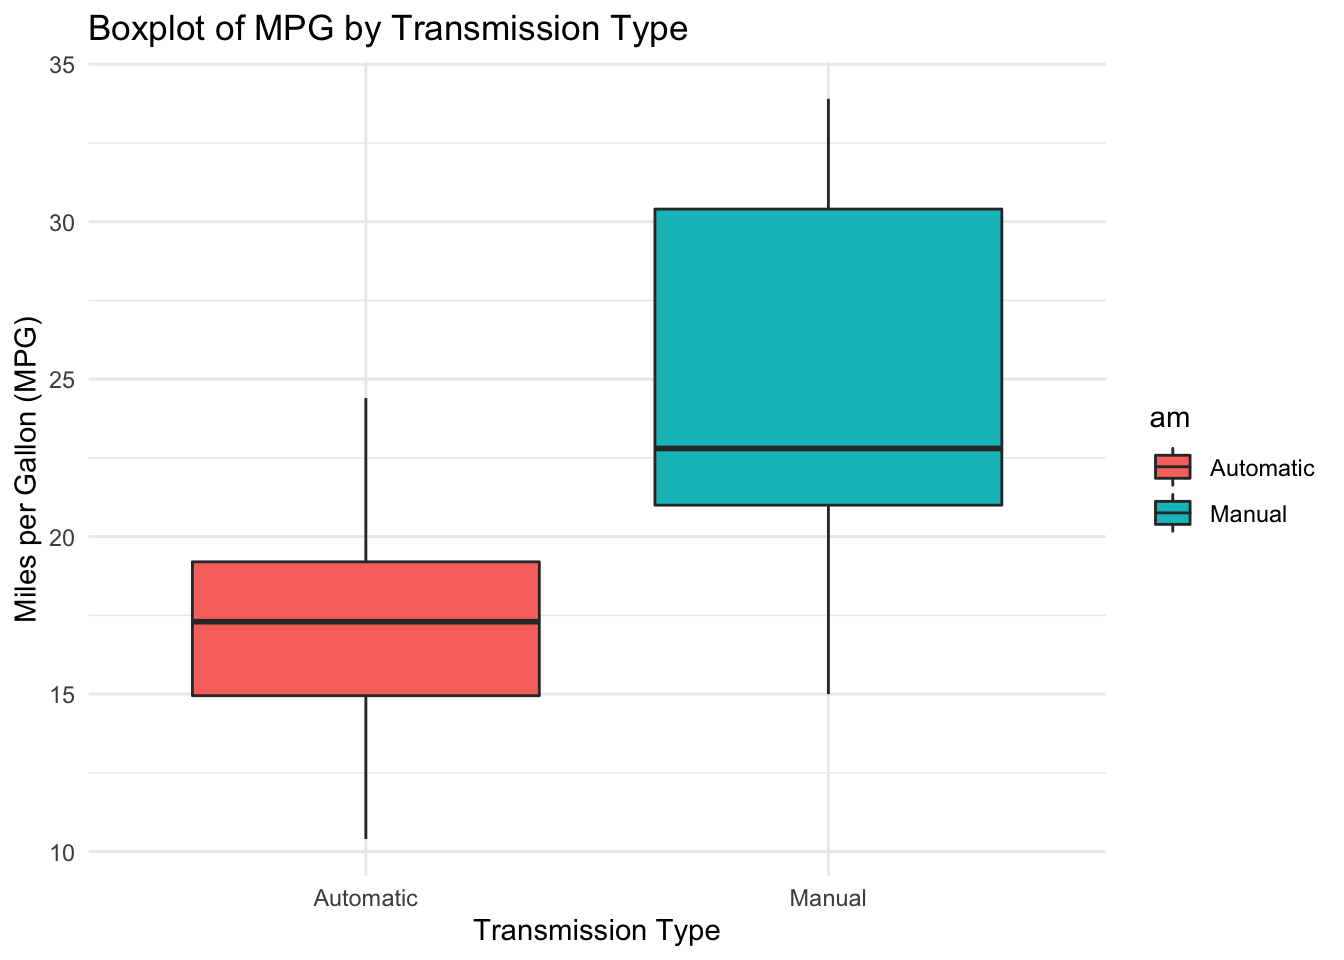
\includegraphics{Lab_sheet3_files/figure-latex/unnamed-chunk-5-1.pdf}

You can also use a matrix whose first column contains x values and
second column contains y values.

\begin{Shaded}
\begin{Highlighting}[]
\NormalTok{M}\OtherTok{\textless{}{-}}\FunctionTok{cbind}\NormalTok{(x.values,y.values)}
\FunctionTok{plot}\NormalTok{(M)}
\end{Highlighting}
\end{Shaded}

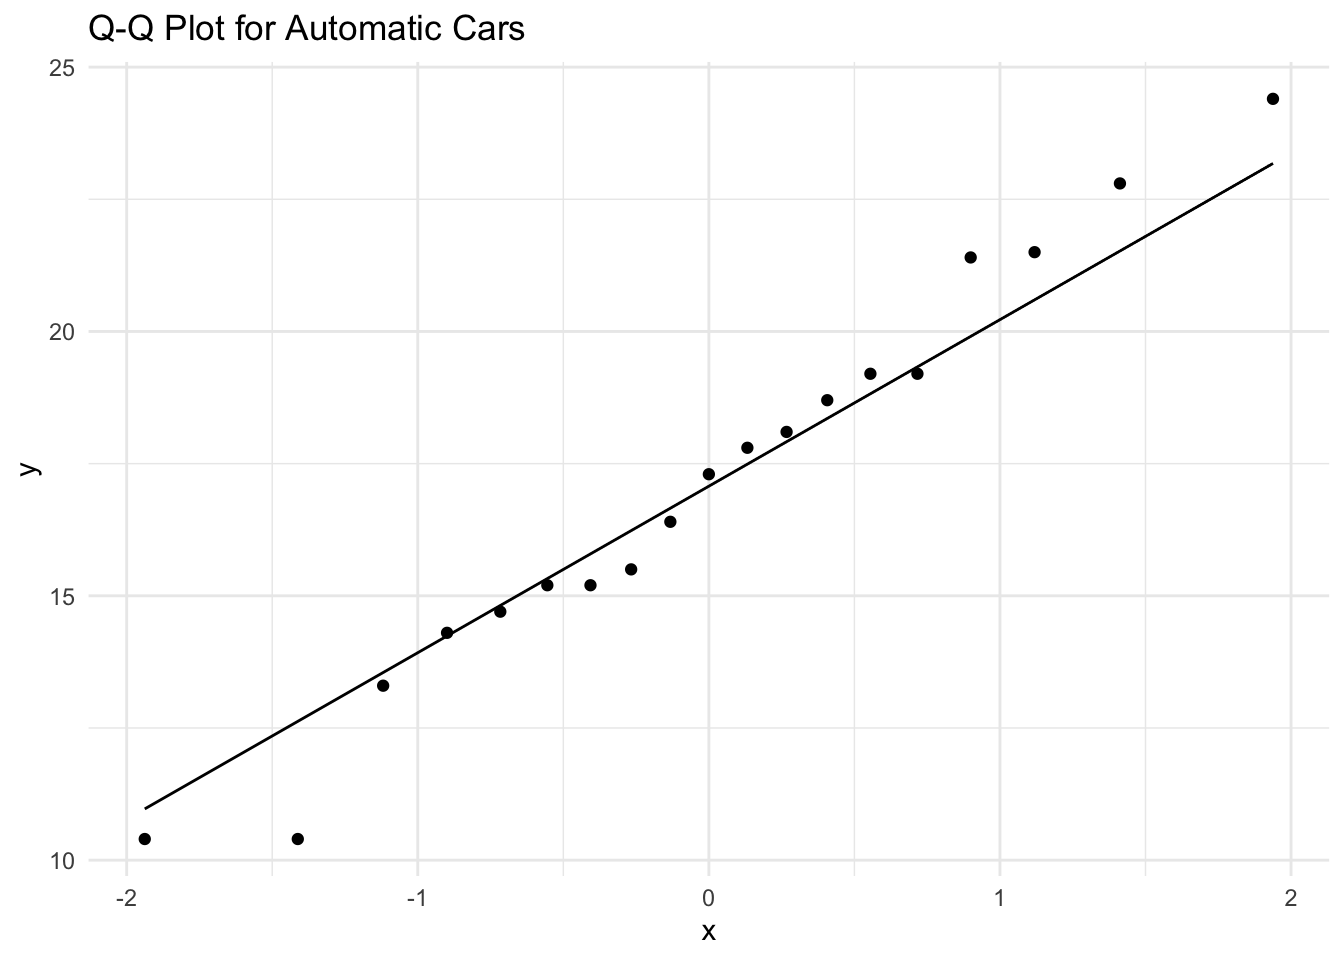
\includegraphics{Lab_sheet3_files/figure-latex/unnamed-chunk-6-1.pdf}

These are some options which can be used in \texttt{plot}.

\begin{center}
    \begin{tabular}{lll}
type&-- & only points or joined by lines or both dots and lines etc.\\
main, xlab, ylab&--& plot title, the horizontal axis label,
the vertical axis label\\
col&--&colors of points and line\\
pch&--&character to use for plotting individual points\\
cex&--&the size of plotted point characters\\
lty&--&type of line (for example, solid, dotted, or dashed)\\
lwd&--&the thickness of plotted lines\\
xlim, ylim&--& horizontal and vertical range of the plotting region
\end{tabular}
\end{center}

To see the options for these parameter type \texttt{?plot} in R console
and click to
\href{https://stat.ethz.ch/R-manual/R-devel/library/base/html/plot.html}{`Generic X-Y Plotting'}.

\hypertarget{examples}{%
\subsubsection{Examples}\label{examples}}

Let us now see some examples:

\begin{Shaded}
\begin{Highlighting}[]
\FunctionTok{plot}\NormalTok{(x.values,y.values,}\AttributeTok{type=}\StringTok{"l"}\NormalTok{)}
\end{Highlighting}
\end{Shaded}

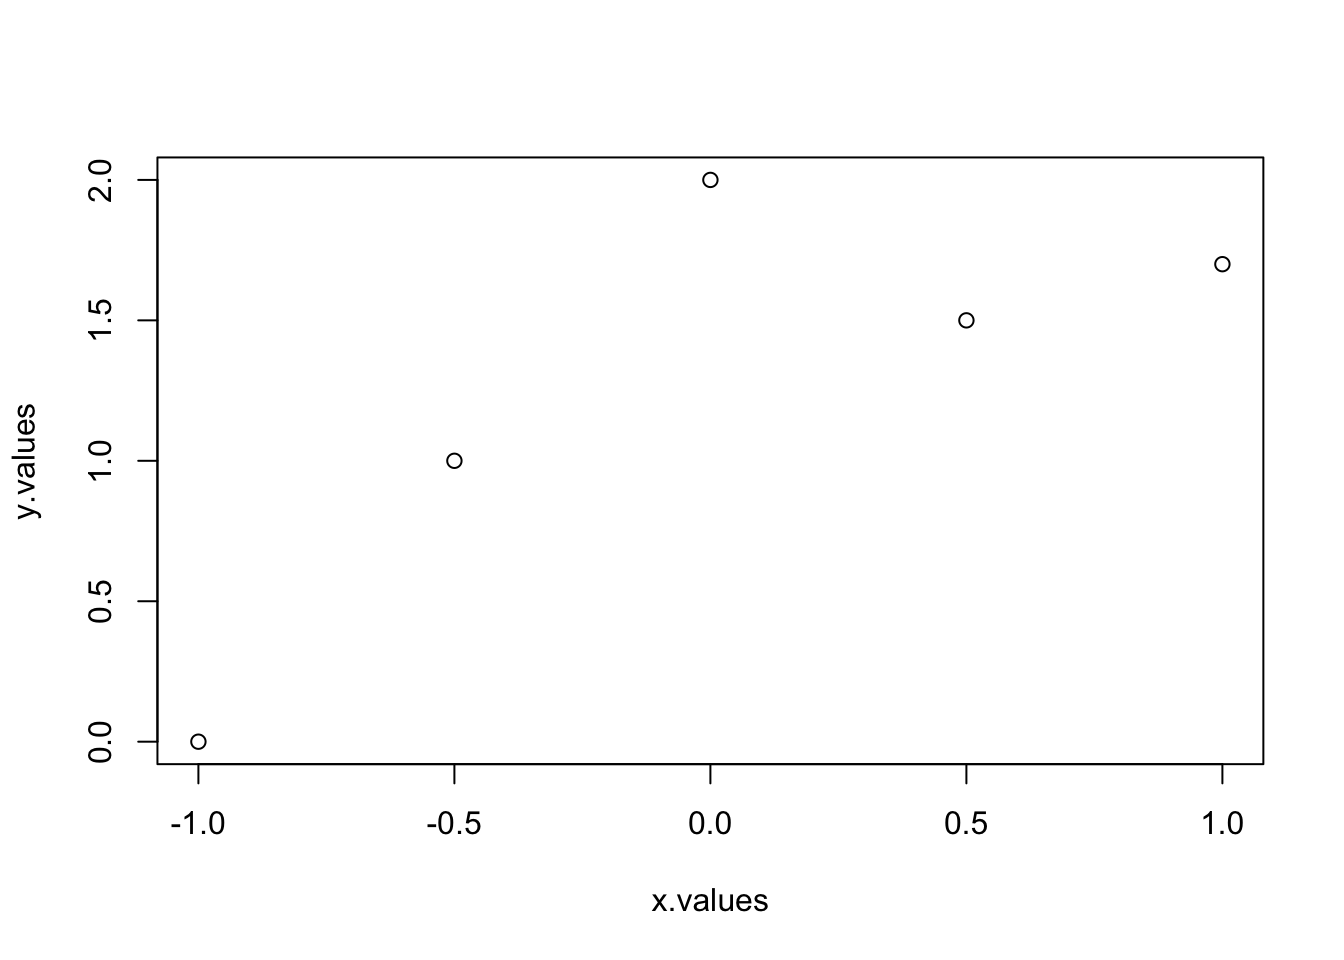
\includegraphics{Lab_sheet3_files/figure-latex/unnamed-chunk-7-1.pdf}

\begin{Shaded}
\begin{Highlighting}[]
\FunctionTok{plot}\NormalTok{(x.values,y.values,}\AttributeTok{type=}\StringTok{"b"}\NormalTok{)}
\end{Highlighting}
\end{Shaded}

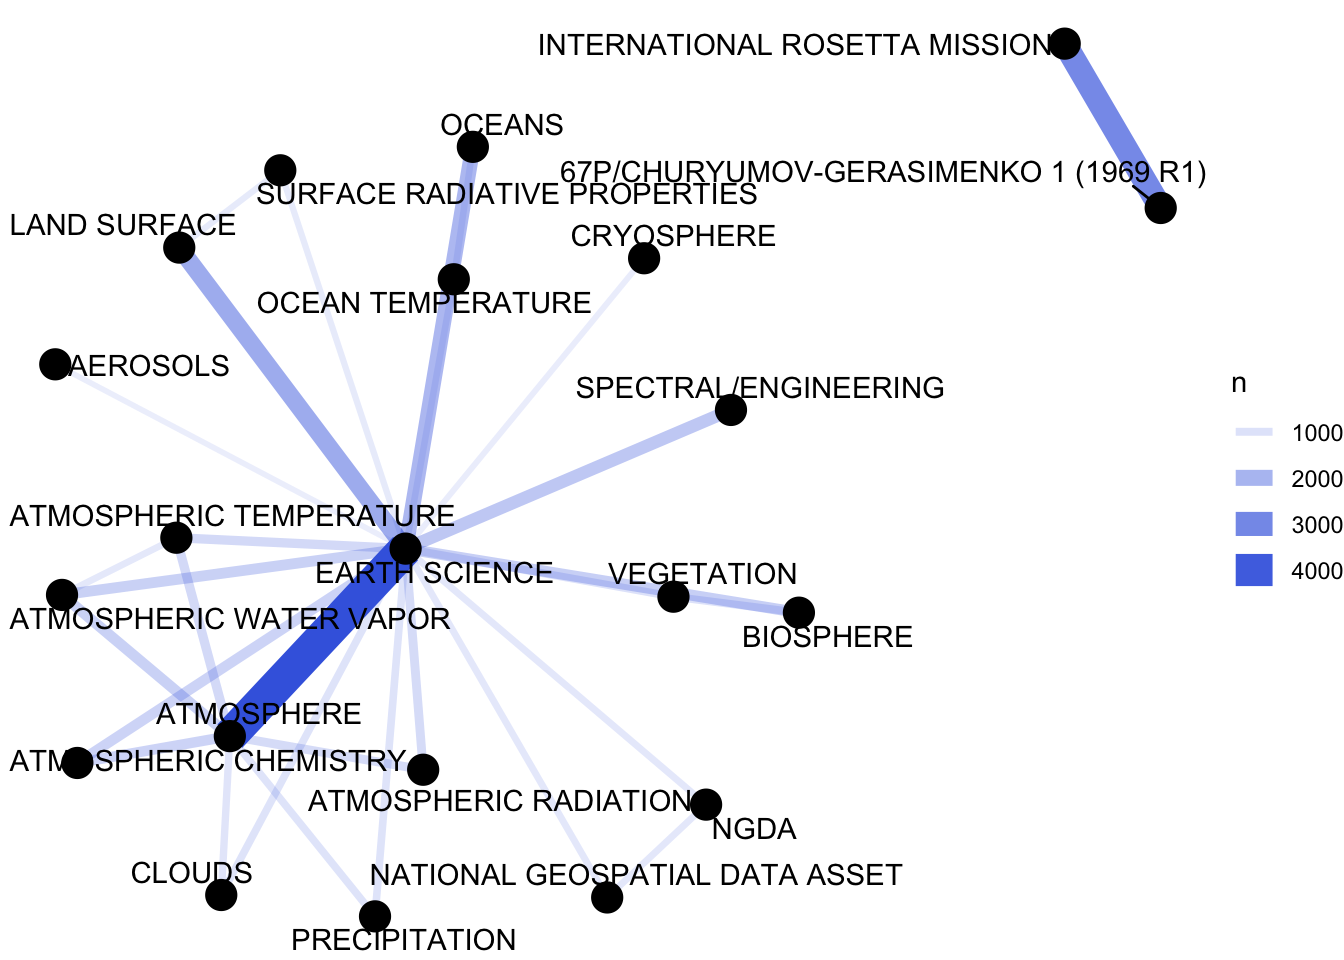
\includegraphics{Lab_sheet3_files/figure-latex/unnamed-chunk-7-2.pdf}

\begin{Shaded}
\begin{Highlighting}[]
\FunctionTok{plot}\NormalTok{(x.values,y.values,}\AttributeTok{type=}\StringTok{"b"}\NormalTok{,}\AttributeTok{main=}\StringTok{"My plot title"}\NormalTok{,}\AttributeTok{xlab=}\StringTok{"x label"}\NormalTok{,}
\AttributeTok{ylab=} \StringTok{"y label"}\NormalTok{)}
\end{Highlighting}
\end{Shaded}

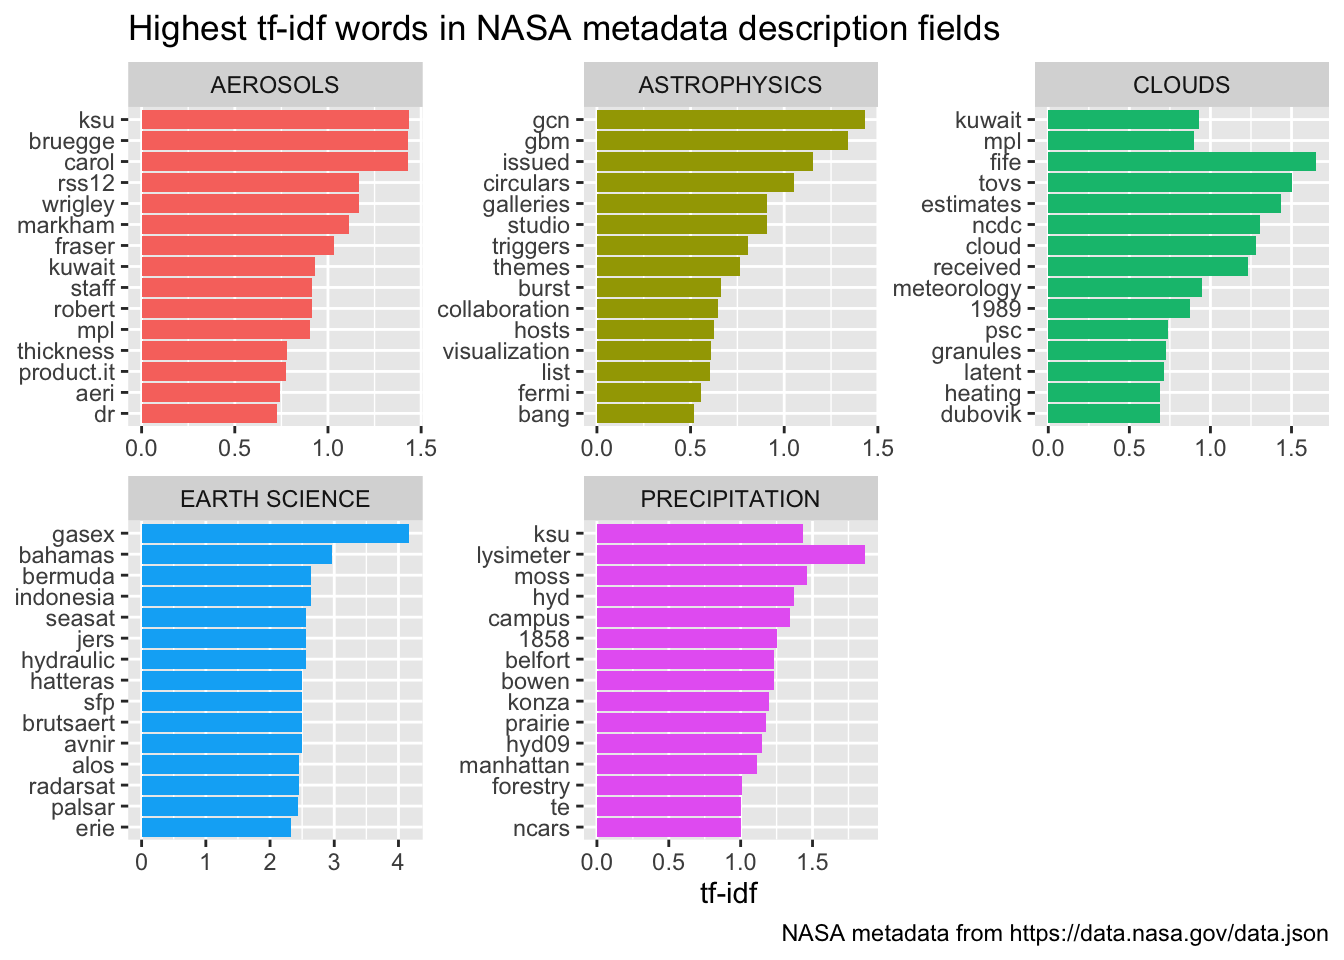
\includegraphics{Lab_sheet3_files/figure-latex/unnamed-chunk-7-3.pdf}

\begin{Shaded}
\begin{Highlighting}[]
\FunctionTok{plot}\NormalTok{(x.values,y.values,}\AttributeTok{type=}\StringTok{"b"}\NormalTok{,}\AttributeTok{main=}\StringTok{"My plot title"}\NormalTok{,}\AttributeTok{xlab=}\StringTok{"x label"}\NormalTok{,}
\AttributeTok{ylab=} \StringTok{"y label"}\NormalTok{,}\AttributeTok{col=}\DecValTok{6}\NormalTok{,}\AttributeTok{pch=}\DecValTok{17}\NormalTok{,}\AttributeTok{lty=}\DecValTok{1}\NormalTok{,}\AttributeTok{cex=}\DecValTok{3}\NormalTok{,}\AttributeTok{lwd=}\DecValTok{2}\NormalTok{,}\AttributeTok{xlim=}\FunctionTok{c}\NormalTok{(}\SpecialCharTok{{-}}\DecValTok{1}\NormalTok{,}\DecValTok{1}\NormalTok{),}\AttributeTok{ylim=}\FunctionTok{c}\NormalTok{(}\DecValTok{0}\NormalTok{,}\DecValTok{2}\NormalTok{))}
\end{Highlighting}
\end{Shaded}

\includegraphics{Lab_sheet3_files/figure-latex/unnamed-chunk-7-4.pdf}

Here are few options for \texttt{pch}:

\begin{center}
    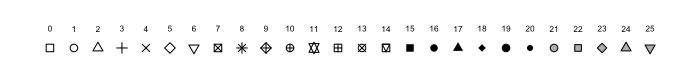
\includegraphics[]{pch}
\end{center}

\hypertarget{adding-points-lines-and-text-in-existing-plots}{%
\subsection{Adding points, lines, and text in existing
plots}\label{adding-points-lines-and-text-in-existing-plots}}

We will see the usage of these commands:

\begin{center}
    \begin{tabular}{lcl}
    points &--& Adds points\\
lines, abline, segments &--& Adds lines\\
text &--& Writes text\\
arrows &--& Adds arrows\\
legend &--& Adds a legend
    \end{tabular}
\end{center}

\begin{Shaded}
\begin{Highlighting}[]
\NormalTok{x }\OtherTok{\textless{}{-}} \FunctionTok{seq}\NormalTok{(}\AttributeTok{from =} \SpecialCharTok{{-}}\DecValTok{1}\NormalTok{, }\AttributeTok{to =} \DecValTok{20}\NormalTok{,  }\AttributeTok{length.out =} \DecValTok{20}\NormalTok{)}
\NormalTok{y }\OtherTok{\textless{}{-}}\NormalTok{ x}\SpecialCharTok{*}\NormalTok{(}\DecValTok{1}\SpecialCharTok{{-}}\FunctionTok{sin}\NormalTok{(}\DecValTok{2}\SpecialCharTok{*}\NormalTok{pi}\SpecialCharTok{*}\NormalTok{x))}
\FunctionTok{plot}\NormalTok{(x,y,}\AttributeTok{type=}\StringTok{"p"}\NormalTok{)}
\end{Highlighting}
\end{Shaded}

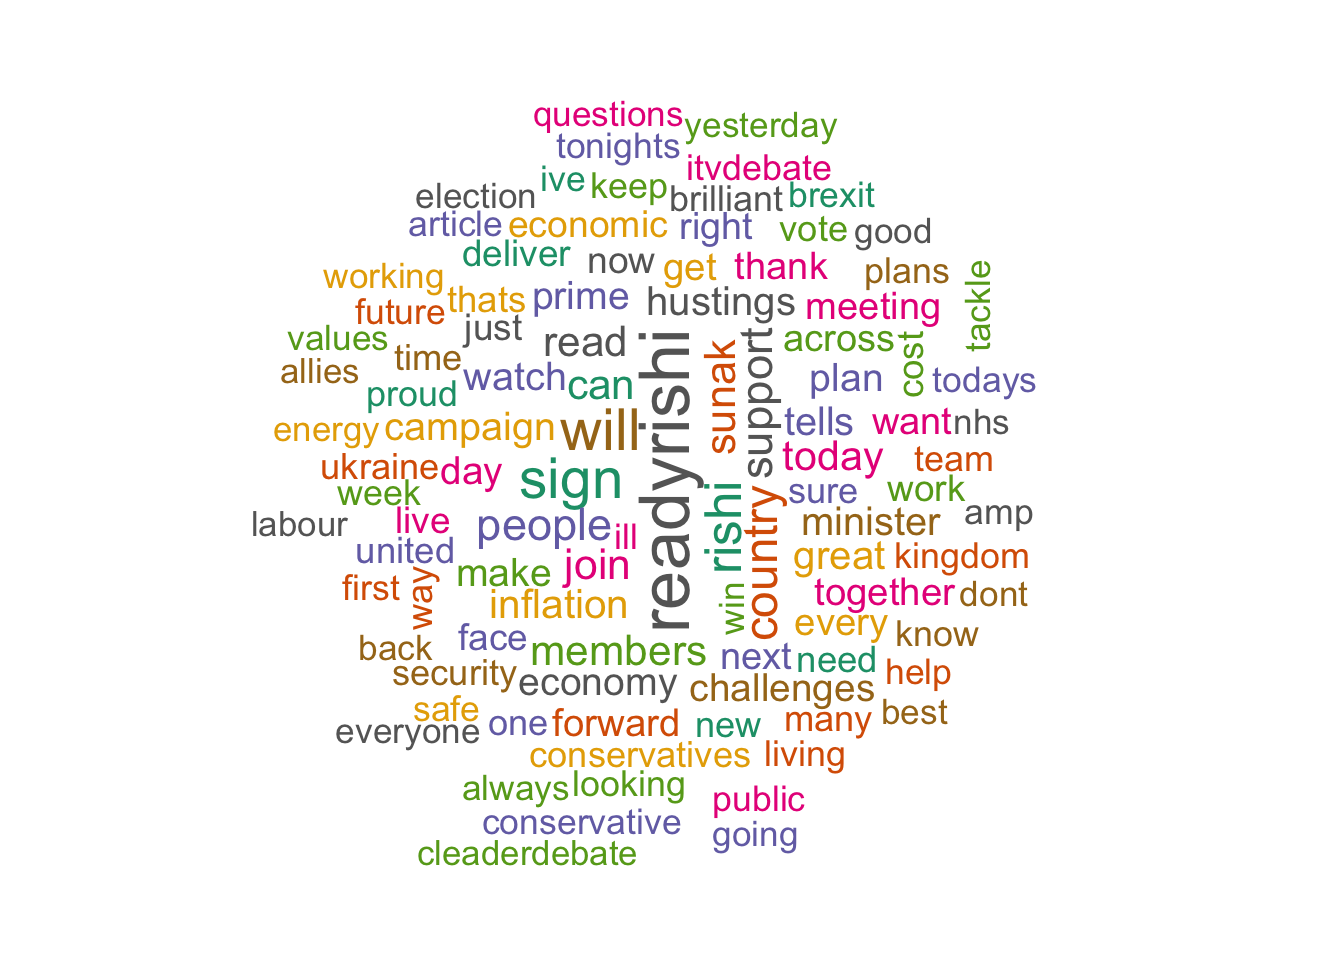
\includegraphics{Lab_sheet3_files/figure-latex/unnamed-chunk-8-1.pdf}

\begin{Shaded}
\begin{Highlighting}[]
\FunctionTok{plot}\NormalTok{(x,y,}\AttributeTok{type=}\StringTok{"p"}\NormalTok{)}
\FunctionTok{abline}\NormalTok{(}\AttributeTok{h=}\FunctionTok{c}\NormalTok{(}\DecValTok{5}\NormalTok{,}\DecValTok{15}\NormalTok{),}\AttributeTok{col=}\StringTok{"red"}\NormalTok{,}\AttributeTok{lty=}\DecValTok{2}\NormalTok{,}\AttributeTok{lwd=}\DecValTok{2}\NormalTok{)}
\FunctionTok{abline}\NormalTok{(}\AttributeTok{a =} \DecValTok{0}\NormalTok{, }\AttributeTok{b =} \DecValTok{1}\NormalTok{, }\AttributeTok{col =} \StringTok{"gray60"}\NormalTok{)}
\FunctionTok{segments}\NormalTok{(}\AttributeTok{x0=}\FunctionTok{c}\NormalTok{(}\DecValTok{5}\NormalTok{,}\DecValTok{15}\NormalTok{),}\AttributeTok{y0=}\FunctionTok{c}\NormalTok{(}\DecValTok{15}\NormalTok{,}\DecValTok{15}\NormalTok{),}\AttributeTok{x1=}\FunctionTok{c}\NormalTok{(}\DecValTok{5}\NormalTok{,}\DecValTok{15}\NormalTok{),}\AttributeTok{y1=}\FunctionTok{c}\NormalTok{(}\DecValTok{5}\NormalTok{,}\DecValTok{5}\NormalTok{),}
\AttributeTok{col=}\DecValTok{4}\NormalTok{,}\AttributeTok{lty=}\DecValTok{4}\NormalTok{,}\AttributeTok{lwd=}\DecValTok{2}\NormalTok{)}
\end{Highlighting}
\end{Shaded}

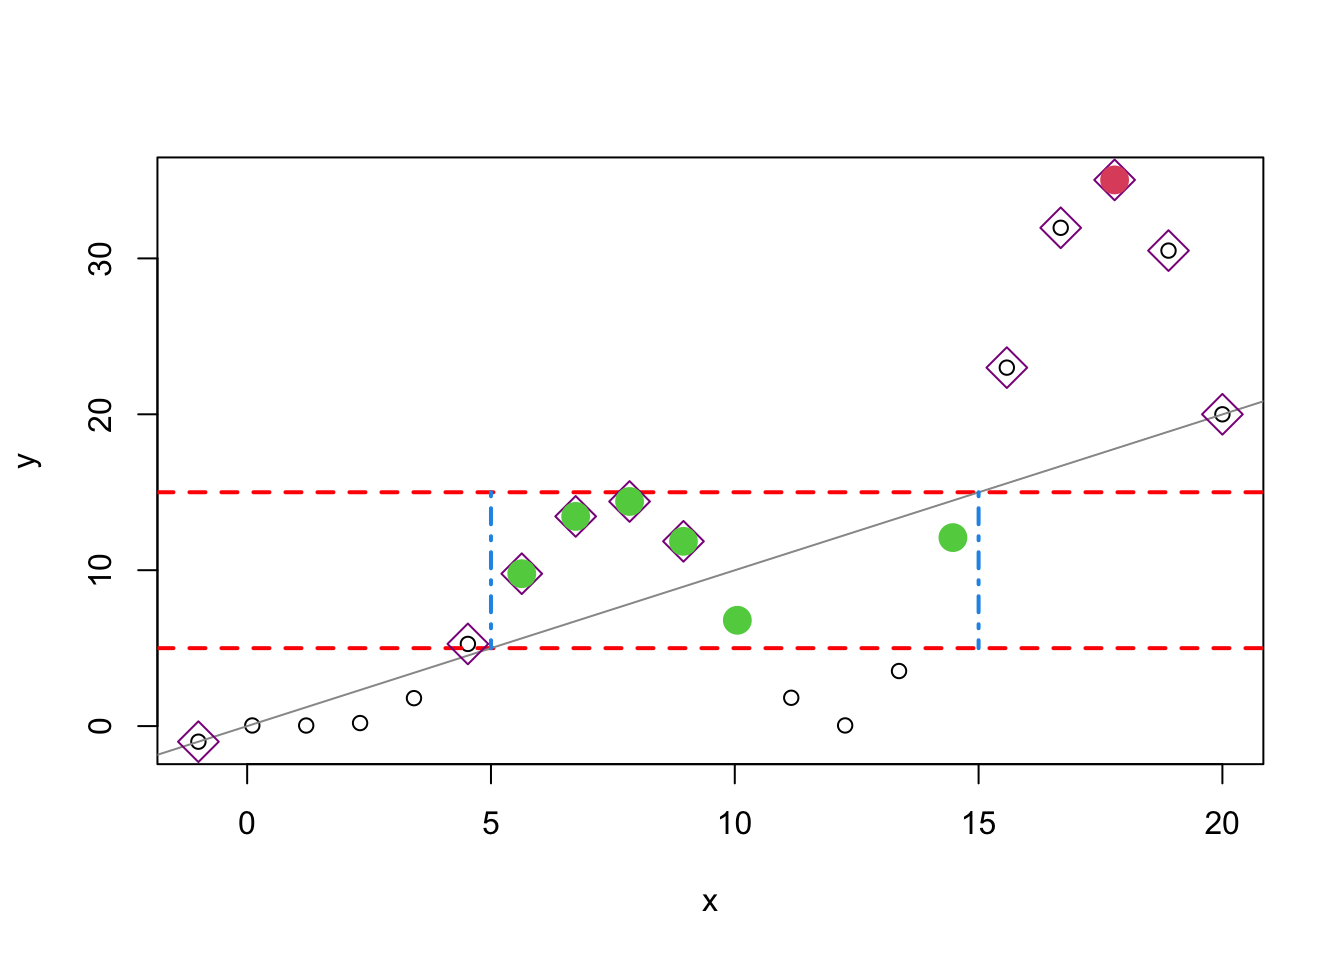
\includegraphics{Lab_sheet3_files/figure-latex/unnamed-chunk-9-1.pdf}

\begin{Shaded}
\begin{Highlighting}[]
\FunctionTok{plot}\NormalTok{(x,y,}\AttributeTok{type=}\StringTok{"p"}\NormalTok{)}
\FunctionTok{abline}\NormalTok{(}\AttributeTok{h=}\FunctionTok{c}\NormalTok{(}\DecValTok{5}\NormalTok{,}\DecValTok{15}\NormalTok{),}\AttributeTok{col=}\StringTok{"red"}\NormalTok{,}\AttributeTok{lty=}\DecValTok{2}\NormalTok{,}\AttributeTok{lwd=}\DecValTok{2}\NormalTok{)}
\FunctionTok{abline}\NormalTok{(}\AttributeTok{a =} \DecValTok{0}\NormalTok{, }\AttributeTok{b =} \DecValTok{1}\NormalTok{, }\AttributeTok{col =} \StringTok{"gray60"}\NormalTok{)}
\FunctionTok{segments}\NormalTok{(}\AttributeTok{x0=}\FunctionTok{c}\NormalTok{(}\DecValTok{5}\NormalTok{,}\DecValTok{15}\NormalTok{),}\AttributeTok{y0=}\FunctionTok{c}\NormalTok{(}\DecValTok{15}\NormalTok{,}\DecValTok{15}\NormalTok{),}\AttributeTok{x1=}\FunctionTok{c}\NormalTok{(}\DecValTok{5}\NormalTok{,}\DecValTok{15}\NormalTok{),}\AttributeTok{y1=}\FunctionTok{c}\NormalTok{(}\DecValTok{5}\NormalTok{,}\DecValTok{5}\NormalTok{),}
\AttributeTok{col=}\DecValTok{4}\NormalTok{,}\AttributeTok{lty=}\DecValTok{4}\NormalTok{,}\AttributeTok{lwd=}\DecValTok{2}\NormalTok{)}
\FunctionTok{points}\NormalTok{(x[x}\SpecialCharTok{\textless{}=}\NormalTok{y],y[x}\SpecialCharTok{\textless{}=}\NormalTok{y],}\AttributeTok{pch=}\DecValTok{5}\NormalTok{,}\AttributeTok{col=}\StringTok{"darkmagenta"}\NormalTok{,}\AttributeTok{cex=}\DecValTok{2}\NormalTok{)}
\FunctionTok{points}\NormalTok{(x[y}\SpecialCharTok{==}\FunctionTok{max}\NormalTok{(y)],y[y}\SpecialCharTok{==}\FunctionTok{max}\NormalTok{(y)],}\AttributeTok{pch=}\DecValTok{16}\NormalTok{,}\AttributeTok{col=}\DecValTok{10}\NormalTok{,}\AttributeTok{cex=}\DecValTok{2}\NormalTok{)}
\FunctionTok{points}\NormalTok{(x[(x}\SpecialCharTok{\textless{}=}\DecValTok{15} \SpecialCharTok{\&}\NormalTok{ x}\SpecialCharTok{\textgreater{}=}\DecValTok{5}\NormalTok{) }\SpecialCharTok{\&}\NormalTok{ (y}\SpecialCharTok{\textless{}=}\DecValTok{15} \SpecialCharTok{\&}\NormalTok{ y}\SpecialCharTok{\textgreater{}=}\DecValTok{5}\NormalTok{)],}
\NormalTok{y[(x}\SpecialCharTok{\textless{}=}\DecValTok{15} \SpecialCharTok{\&}\NormalTok{ x}\SpecialCharTok{\textgreater{}=}\DecValTok{5}\NormalTok{) }\SpecialCharTok{\&}\NormalTok{ (y}\SpecialCharTok{\textless{}=}\DecValTok{15} \SpecialCharTok{\&}\NormalTok{ y}\SpecialCharTok{\textgreater{}=}\DecValTok{5}\NormalTok{)],}\AttributeTok{pch=}\DecValTok{16}\NormalTok{,}\AttributeTok{col=}\DecValTok{3}\NormalTok{,}\AttributeTok{cex=}\DecValTok{2}\NormalTok{)}
\end{Highlighting}
\end{Shaded}

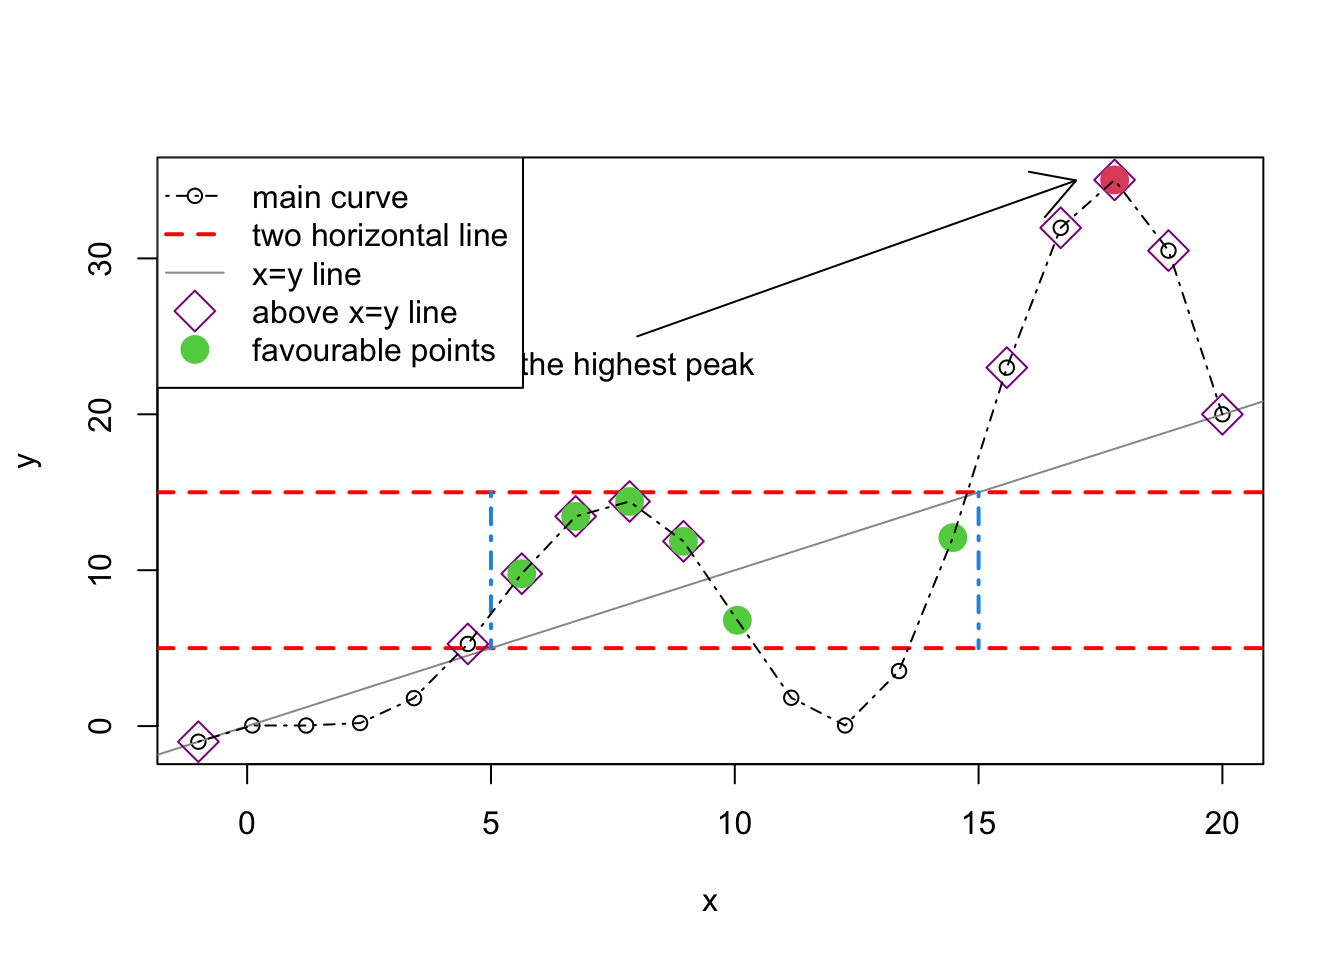
\includegraphics{Lab_sheet3_files/figure-latex/unnamed-chunk-10-1.pdf}

\begin{Shaded}
\begin{Highlighting}[]
\FunctionTok{plot}\NormalTok{(x,y,}\AttributeTok{type=}\StringTok{"p"}\NormalTok{)}
\FunctionTok{abline}\NormalTok{(}\AttributeTok{h=}\FunctionTok{c}\NormalTok{(}\DecValTok{5}\NormalTok{,}\DecValTok{15}\NormalTok{),}\AttributeTok{col=}\StringTok{"red"}\NormalTok{,}\AttributeTok{lty=}\DecValTok{2}\NormalTok{,}\AttributeTok{lwd=}\DecValTok{2}\NormalTok{)}
\FunctionTok{abline}\NormalTok{(}\AttributeTok{a =} \DecValTok{0}\NormalTok{, }\AttributeTok{b =} \DecValTok{1}\NormalTok{, }\AttributeTok{col =} \StringTok{"gray60"}\NormalTok{)}
\FunctionTok{segments}\NormalTok{(}\AttributeTok{x0=}\FunctionTok{c}\NormalTok{(}\DecValTok{5}\NormalTok{,}\DecValTok{15}\NormalTok{),}\AttributeTok{y0=}\FunctionTok{c}\NormalTok{(}\DecValTok{15}\NormalTok{,}\DecValTok{15}\NormalTok{),}\AttributeTok{x1=}\FunctionTok{c}\NormalTok{(}\DecValTok{5}\NormalTok{,}\DecValTok{15}\NormalTok{),}\AttributeTok{y1=}\FunctionTok{c}\NormalTok{(}\DecValTok{5}\NormalTok{,}\DecValTok{5}\NormalTok{),}
\AttributeTok{col=}\DecValTok{4}\NormalTok{,}\AttributeTok{lty=}\DecValTok{4}\NormalTok{,}\AttributeTok{lwd=}\DecValTok{2}\NormalTok{)}
\FunctionTok{points}\NormalTok{(x[x}\SpecialCharTok{\textless{}=}\NormalTok{y],y[x}\SpecialCharTok{\textless{}=}\NormalTok{y],}\AttributeTok{pch=}\DecValTok{5}\NormalTok{,}\AttributeTok{col=}\StringTok{"darkmagenta"}\NormalTok{,}\AttributeTok{cex=}\DecValTok{2}\NormalTok{)}
\FunctionTok{points}\NormalTok{(x[y}\SpecialCharTok{==}\FunctionTok{max}\NormalTok{(y)],y[y}\SpecialCharTok{==}\FunctionTok{max}\NormalTok{(y)],}\AttributeTok{pch=}\DecValTok{16}\NormalTok{,}\AttributeTok{col=}\DecValTok{10}\NormalTok{,}\AttributeTok{cex=}\DecValTok{2}\NormalTok{)}
\FunctionTok{points}\NormalTok{(x[(x}\SpecialCharTok{\textless{}=}\DecValTok{15} \SpecialCharTok{\&}\NormalTok{ x}\SpecialCharTok{\textgreater{}=}\DecValTok{5}\NormalTok{) }\SpecialCharTok{\&}\NormalTok{ (y}\SpecialCharTok{\textless{}=}\DecValTok{15} \SpecialCharTok{\&}\NormalTok{ y}\SpecialCharTok{\textgreater{}=}\DecValTok{5}\NormalTok{)],}
\NormalTok{y[(x}\SpecialCharTok{\textless{}=}\DecValTok{15} \SpecialCharTok{\&}\NormalTok{ x}\SpecialCharTok{\textgreater{}=}\DecValTok{5}\NormalTok{) }\SpecialCharTok{\&}\NormalTok{ (y}\SpecialCharTok{\textless{}=}\DecValTok{15} \SpecialCharTok{\&}\NormalTok{ y}\SpecialCharTok{\textgreater{}=}\DecValTok{5}\NormalTok{)],}\AttributeTok{pch=}\DecValTok{16}\NormalTok{,}\AttributeTok{col=}\DecValTok{3}\NormalTok{,}\AttributeTok{cex=}\DecValTok{2}\NormalTok{)}
\FunctionTok{lines}\NormalTok{(x,y,}\AttributeTok{lty=}\DecValTok{4}\NormalTok{)}
\FunctionTok{arrows}\NormalTok{(}\AttributeTok{x0=}\DecValTok{8}\NormalTok{,}\AttributeTok{y0=}\DecValTok{25}\NormalTok{,}\AttributeTok{x1=}\DecValTok{17}\NormalTok{,}\AttributeTok{y1=}\DecValTok{35}\NormalTok{)}
\FunctionTok{text}\NormalTok{(}\AttributeTok{x=}\DecValTok{8}\NormalTok{,}\AttributeTok{y=}\DecValTok{25}\NormalTok{,}\AttributeTok{pos=}\DecValTok{1}\NormalTok{,}\AttributeTok{labels=}\StringTok{"the highest peak"}\NormalTok{)}
\FunctionTok{legend}\NormalTok{(}\StringTok{"topleft"}\NormalTok{,}
\AttributeTok{legend=}\FunctionTok{c}\NormalTok{(}\StringTok{"main curve"}\NormalTok{,}\StringTok{"two horizontal line"}\NormalTok{,}\StringTok{"x=y line"}\NormalTok{,}
\StringTok{"above x=y line"}\NormalTok{,}\StringTok{"favourable points"}\NormalTok{),}\AttributeTok{pch=}\FunctionTok{c}\NormalTok{(}\DecValTok{1}\NormalTok{,}\ConstantTok{NA}\NormalTok{,}\ConstantTok{NA}\NormalTok{,}\DecValTok{5}\NormalTok{,}\DecValTok{16}\NormalTok{),}\AttributeTok{lty=}\FunctionTok{c}\NormalTok{(}\DecValTok{4}\NormalTok{,}\DecValTok{2}\NormalTok{,}\DecValTok{1}\NormalTok{,}\ConstantTok{NA}\NormalTok{,}\ConstantTok{NA}\NormalTok{),}
\AttributeTok{col=}\FunctionTok{c}\NormalTok{(}\StringTok{"black"}\NormalTok{,}\StringTok{"red"}\NormalTok{,}\StringTok{"gray60"}\NormalTok{,}\StringTok{"darkmagenta"}\NormalTok{,}\DecValTok{3}\NormalTok{),}
\AttributeTok{lwd=}\FunctionTok{c}\NormalTok{(}\DecValTok{1}\NormalTok{,}\DecValTok{2}\NormalTok{,}\DecValTok{1}\NormalTok{,}\DecValTok{1}\NormalTok{,}\ConstantTok{NA}\NormalTok{),}\AttributeTok{pt.cex=}\FunctionTok{c}\NormalTok{(}\DecValTok{1}\NormalTok{,}\ConstantTok{NA}\NormalTok{,}\ConstantTok{NA}\NormalTok{,}\DecValTok{2}\NormalTok{,}\DecValTok{2}\NormalTok{))}
\end{Highlighting}
\end{Shaded}

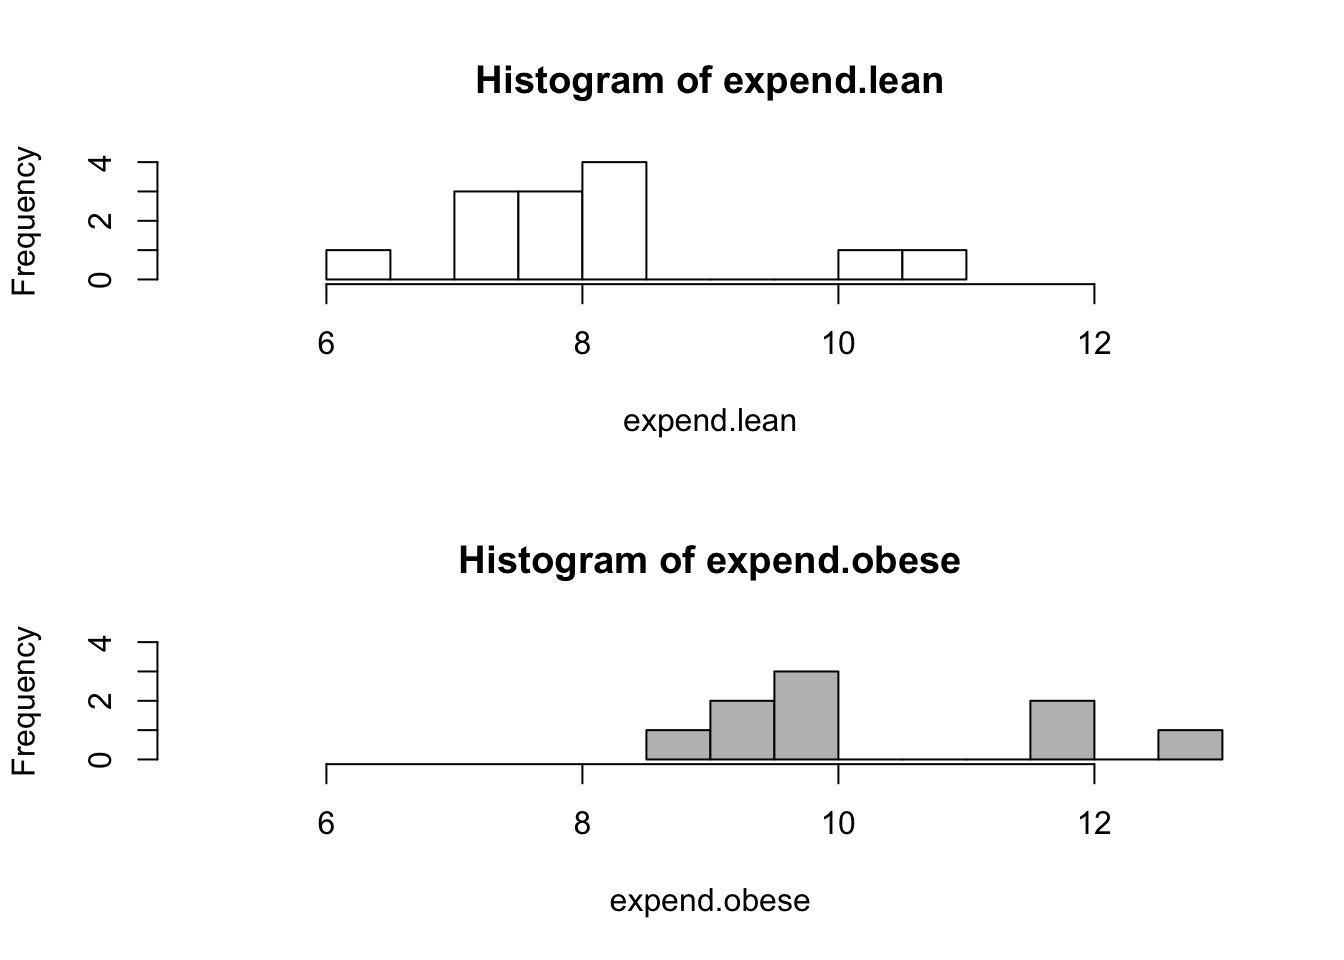
\includegraphics{Lab_sheet3_files/figure-latex/unnamed-chunk-11-1.pdf}

\hypertarget{shading-between-curves}{%
\subsection{Shading between curves}\label{shading-between-curves}}

\begin{Shaded}
\begin{Highlighting}[]
\NormalTok{x1}\OtherTok{=}\FunctionTok{seq}\NormalTok{(}\AttributeTok{from=}\SpecialCharTok{{-}}\NormalTok{pi,}\AttributeTok{to=}\NormalTok{pi,}\AttributeTok{length.out =}\DecValTok{100}\NormalTok{)}
\NormalTok{y1 }\OtherTok{\textless{}{-}} \FunctionTok{sin}\NormalTok{(x1) }
\NormalTok{y2 }\OtherTok{\textless{}{-}} \FunctionTok{cos}\NormalTok{(x1)}
\FunctionTok{plot}\NormalTok{(x1,y1,}\AttributeTok{type=}\StringTok{"l"}\NormalTok{,}\AttributeTok{bty=}\StringTok{"L"}\NormalTok{,}\AttributeTok{xlab=}\StringTok{"x"}\NormalTok{,}\AttributeTok{ylab=}\StringTok{"y"}\NormalTok{,}\AttributeTok{col=}\DecValTok{4}\NormalTok{)}
\FunctionTok{points}\NormalTok{(x1,y2,}\AttributeTok{type=}\StringTok{"l"}\NormalTok{,}\AttributeTok{col=}\StringTok{"red"}\NormalTok{)}
\FunctionTok{polygon}\NormalTok{(}\FunctionTok{c}\NormalTok{(x1,}\FunctionTok{rev}\NormalTok{(x1)),}\FunctionTok{c}\NormalTok{(y2,}\FunctionTok{rev}\NormalTok{(y1)),}\AttributeTok{col=}\FunctionTok{gray}\NormalTok{(}\FloatTok{0.8}\NormalTok{))}
\end{Highlighting}
\end{Shaded}

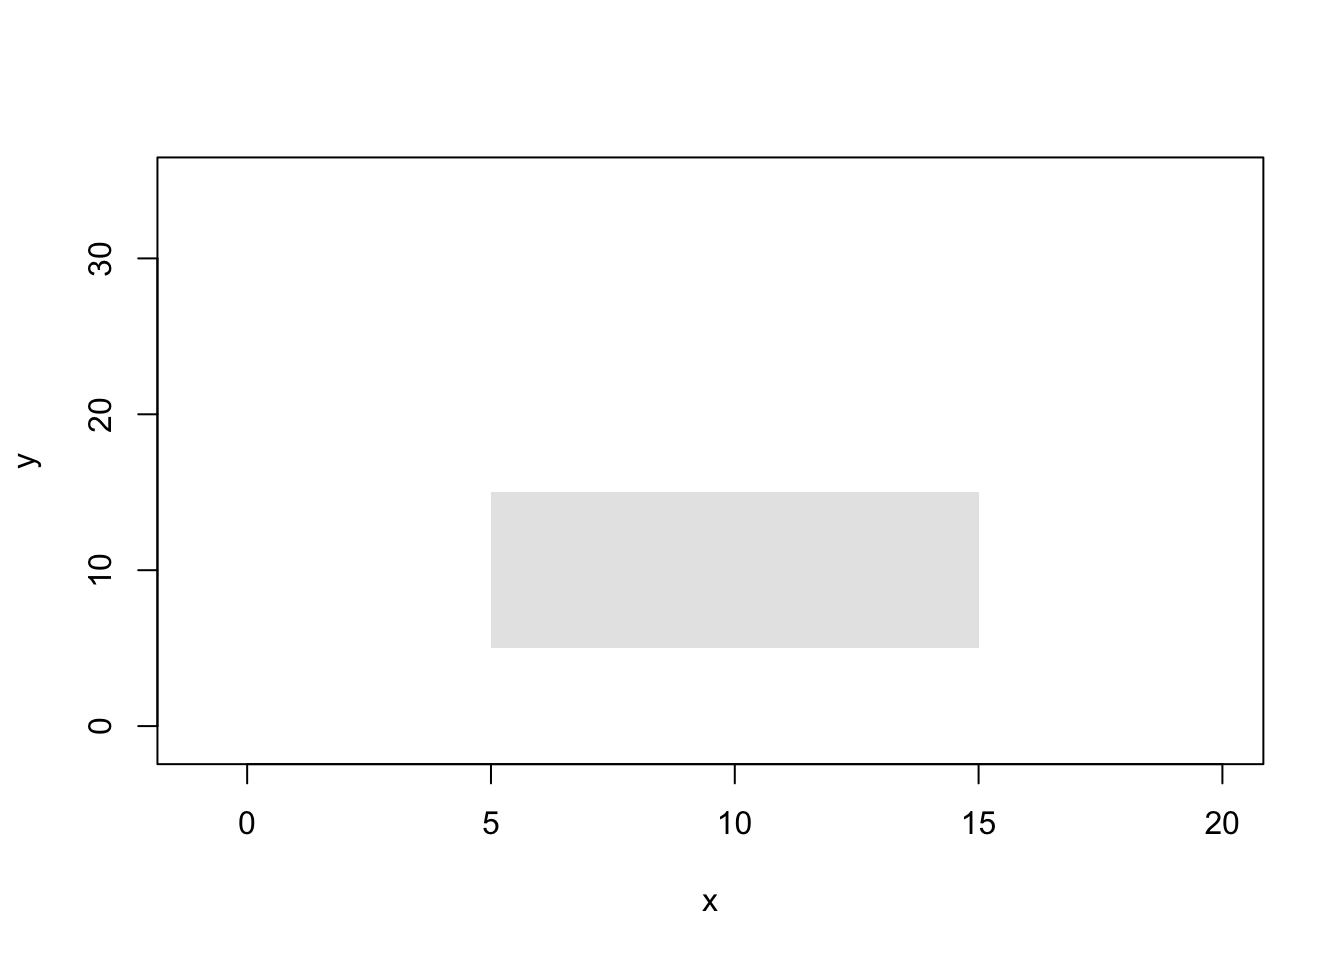
\includegraphics{Lab_sheet3_files/figure-latex/unnamed-chunk-12-1.pdf}

\begin{Shaded}
\begin{Highlighting}[]
\FunctionTok{plot}\NormalTok{(x,y,}\AttributeTok{type=}\StringTok{"n"}\NormalTok{)}
\FunctionTok{rect}\NormalTok{(}\DecValTok{5}\NormalTok{, }\DecValTok{5}\NormalTok{, }\DecValTok{15}\NormalTok{, }\DecValTok{15}\NormalTok{, }\AttributeTok{col=}\FunctionTok{gray}\NormalTok{(}\FloatTok{0.9}\NormalTok{), }\AttributeTok{border=}\ConstantTok{NA}\NormalTok{)}
\end{Highlighting}
\end{Shaded}

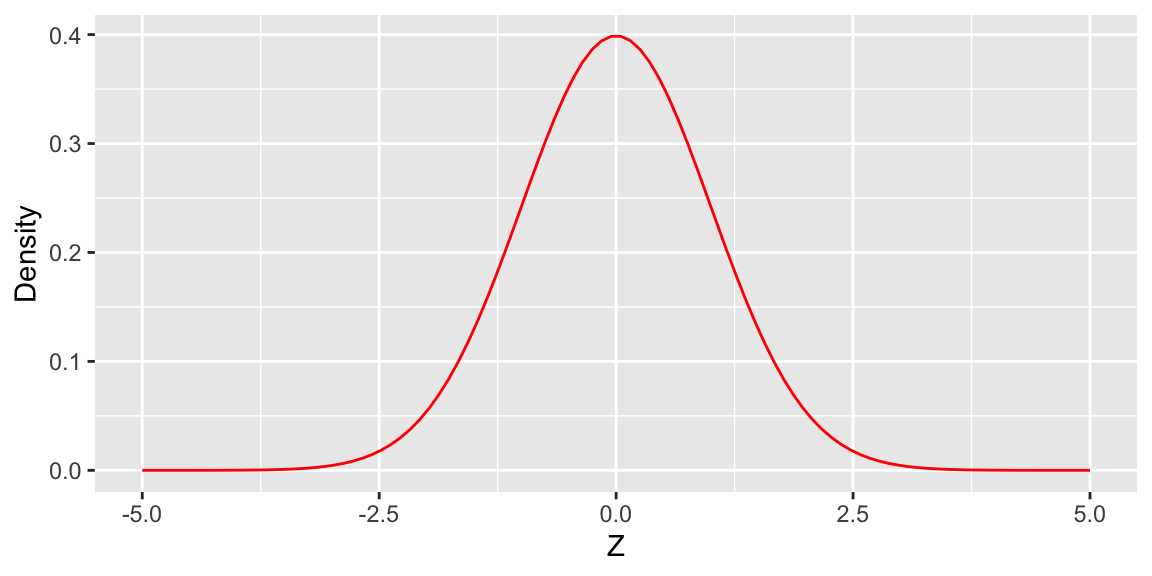
\includegraphics{Lab_sheet3_files/figure-latex/unnamed-chunk-13-1.pdf}
\#\#\# Packages other than R base There are few good R packages for data
visualisation: ggplot2, Lattice, Plotly and few more. Let us explore
ggplot2 a bit. First, use install.packages(``ggplot2'') to install.

\begin{Shaded}
\begin{Highlighting}[]
\FunctionTok{library}\NormalTok{(}\StringTok{"ggplot2"}\NormalTok{)}
\FunctionTok{qplot}\NormalTok{(x.values,y.values)}
\end{Highlighting}
\end{Shaded}

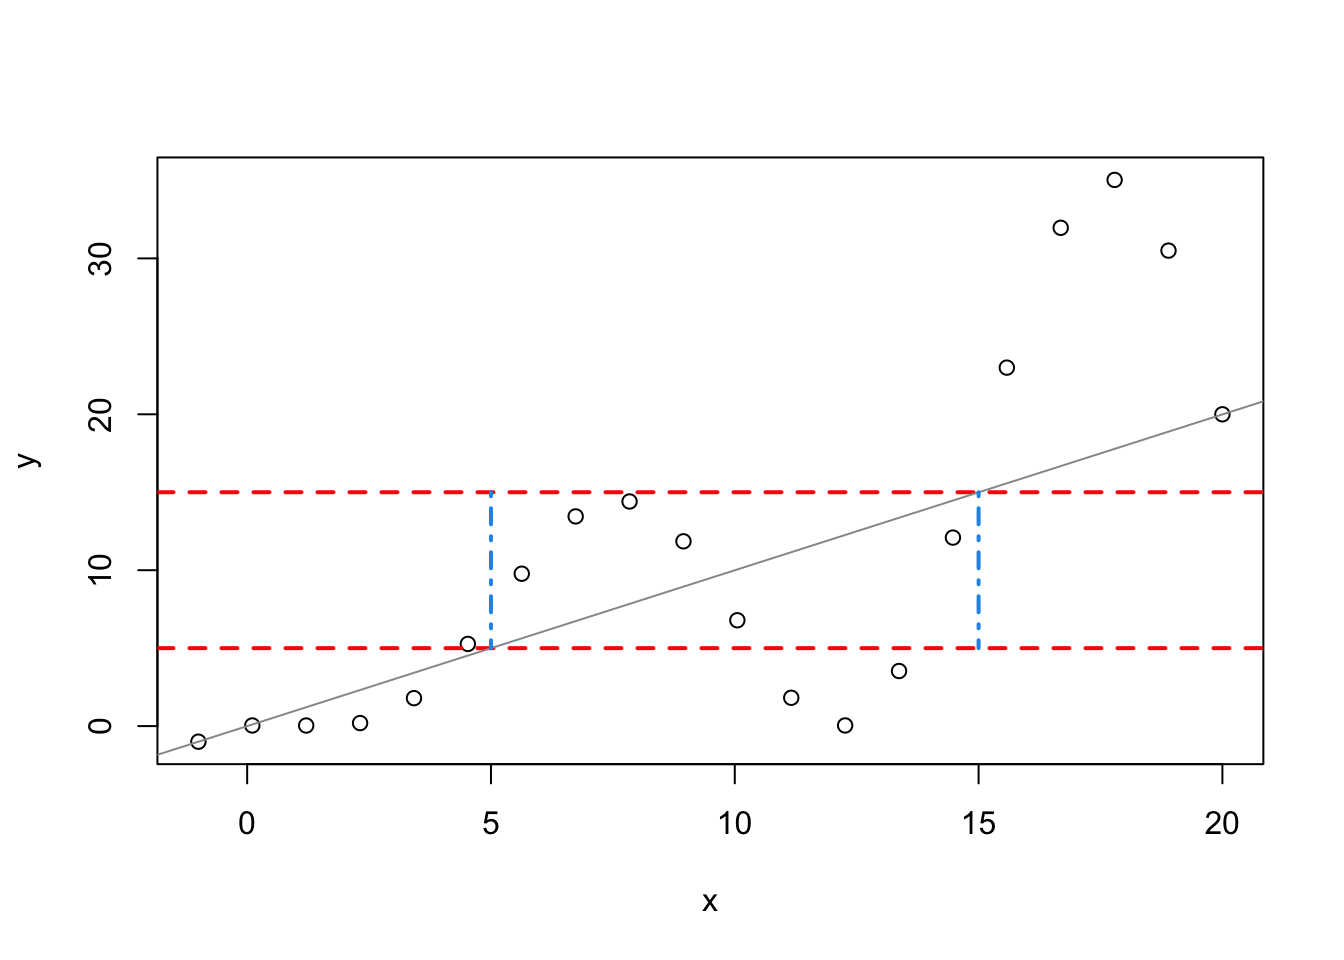
\includegraphics{Lab_sheet3_files/figure-latex/unnamed-chunk-14-1.pdf}

\begin{Shaded}
\begin{Highlighting}[]
\FunctionTok{qplot}\NormalTok{(x.values,y.values,}\AttributeTok{main=}\StringTok{"My qplot"}\NormalTok{,}\AttributeTok{xlab=}\StringTok{"x label"}\NormalTok{,}
\AttributeTok{ylab=} \StringTok{"y label"}\NormalTok{)}
\end{Highlighting}
\end{Shaded}

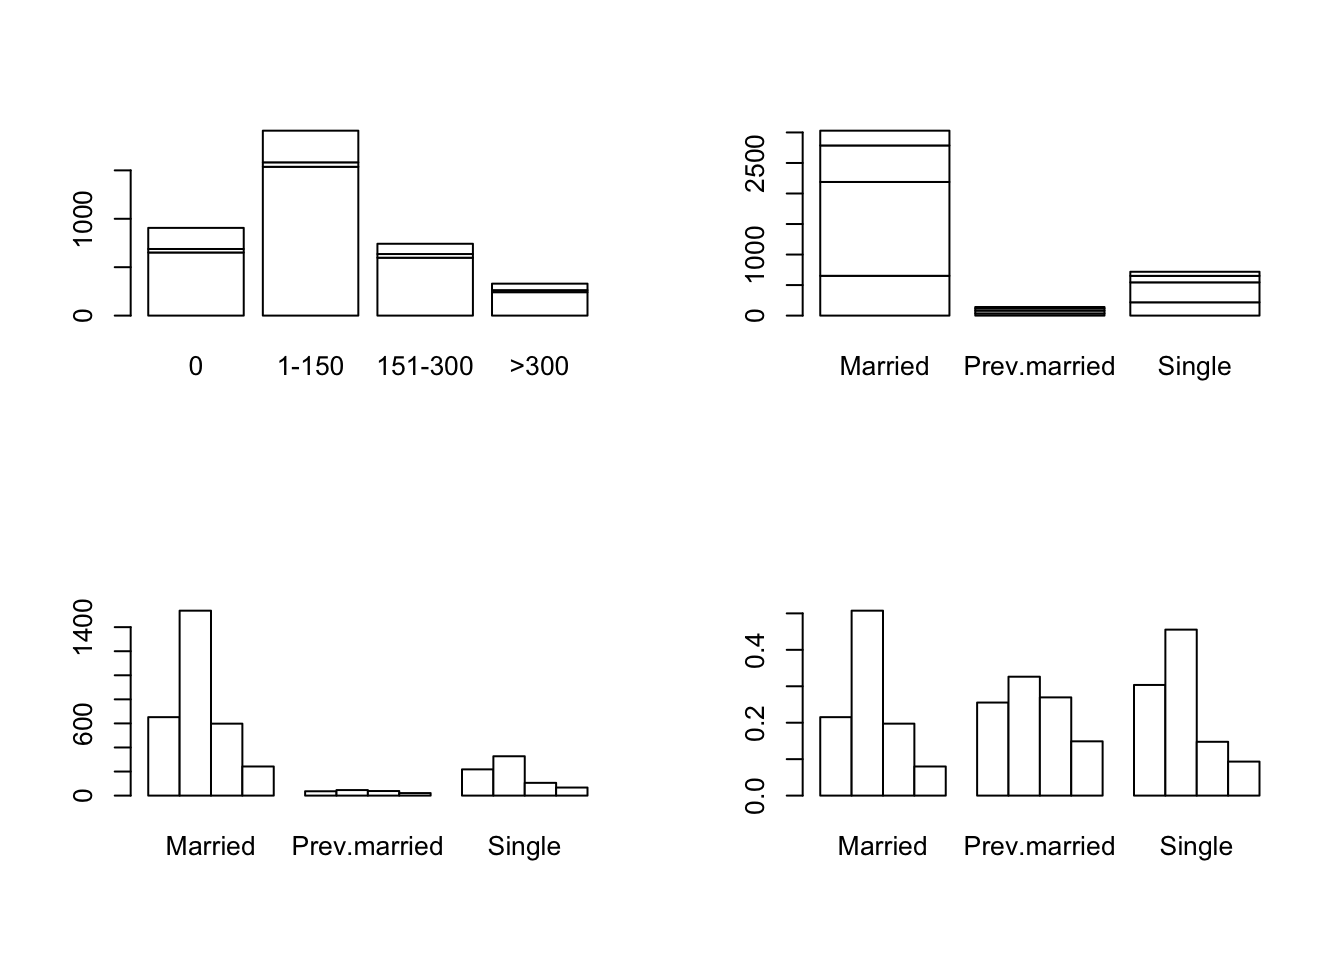
\includegraphics{Lab_sheet3_files/figure-latex/unnamed-chunk-14-2.pdf}

\begin{Shaded}
\begin{Highlighting}[]
\NormalTok{h}\OtherTok{=}\FunctionTok{qplot}\NormalTok{(x.values,y.values)}
\NormalTok{h}
\end{Highlighting}
\end{Shaded}

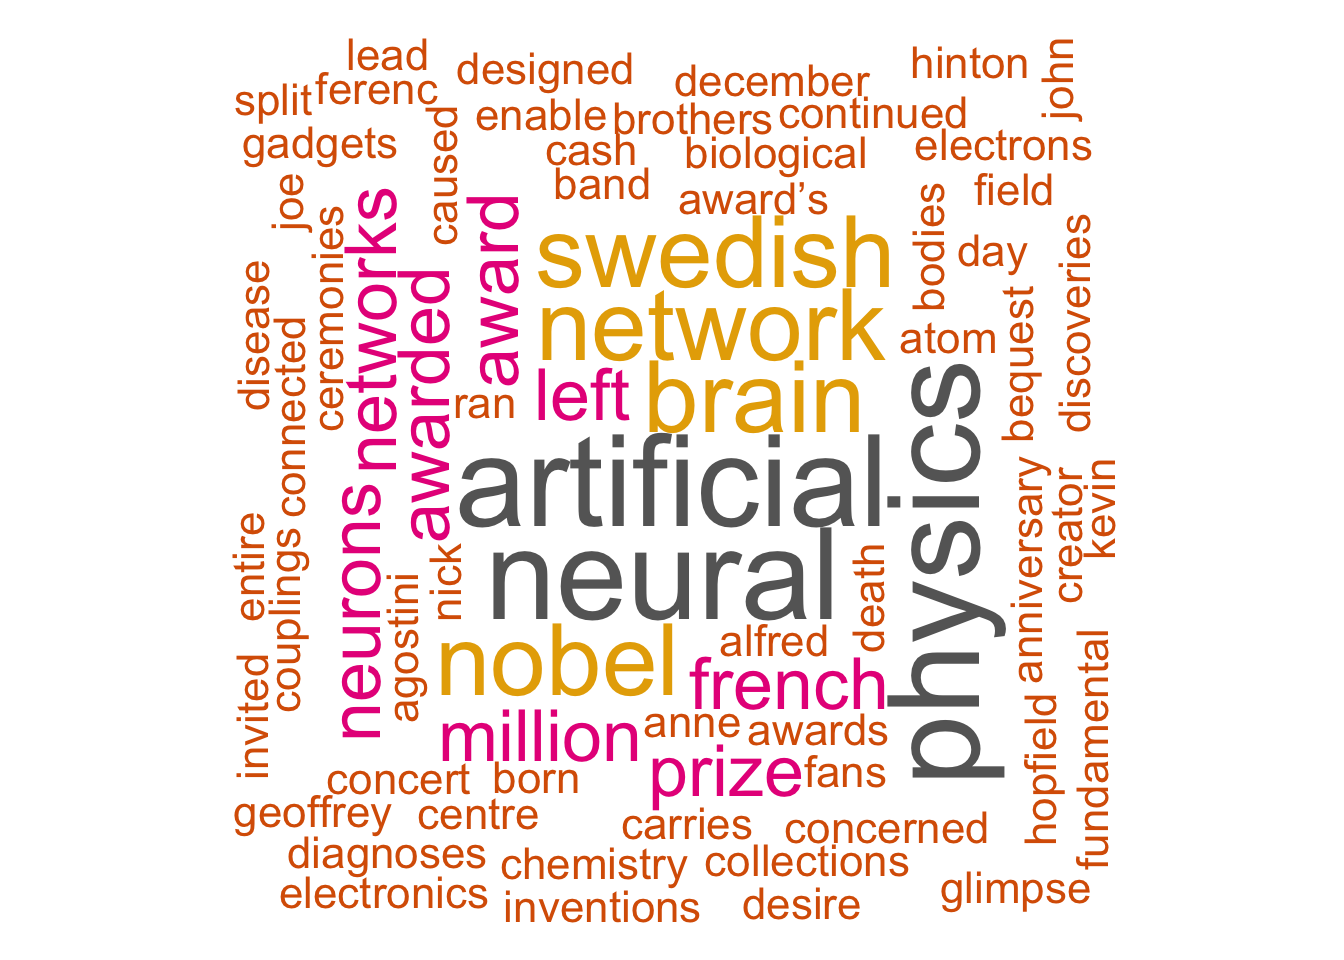
\includegraphics{Lab_sheet3_files/figure-latex/unnamed-chunk-15-1.pdf}

\begin{Shaded}
\begin{Highlighting}[]
\FunctionTok{qplot}\NormalTok{(x,y,}\AttributeTok{geom=}\StringTok{"blank"}\NormalTok{) }\SpecialCharTok{+} \FunctionTok{geom\_point}\NormalTok{() }\SpecialCharTok{+} \FunctionTok{geom\_line}\NormalTok{()}
\end{Highlighting}
\end{Shaded}

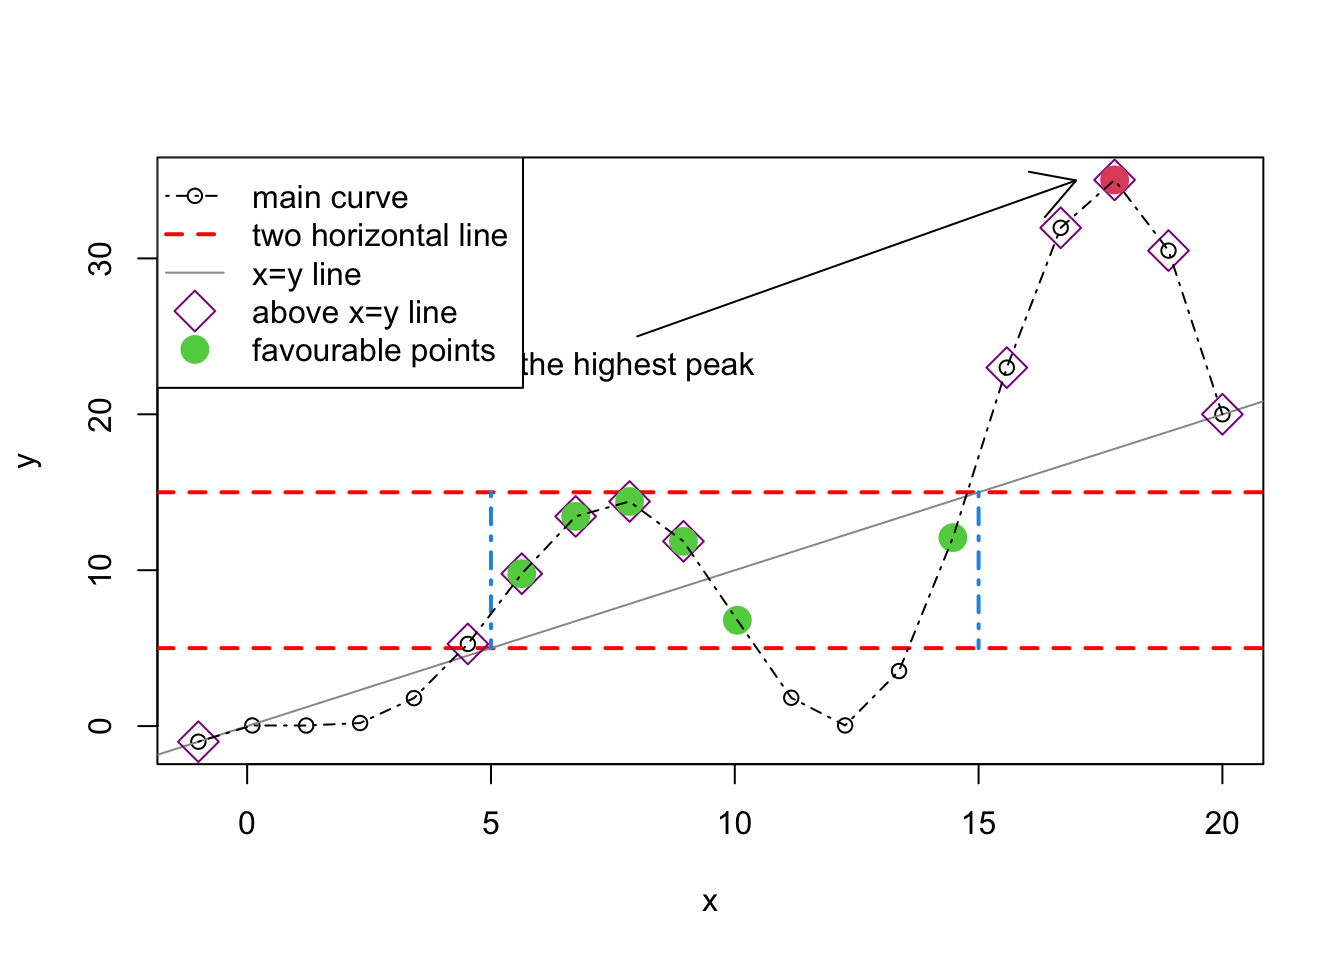
\includegraphics{Lab_sheet3_files/figure-latex/unnamed-chunk-16-1.pdf}

\begin{Shaded}
\begin{Highlighting}[]
\NormalTok{myqplot }\OtherTok{\textless{}{-}} \FunctionTok{qplot}\NormalTok{(x,y,}\AttributeTok{geom=}\StringTok{"blank"}\NormalTok{) }\SpecialCharTok{+} \FunctionTok{geom\_line}\NormalTok{(}\AttributeTok{color=}\StringTok{"red"}\NormalTok{,}\AttributeTok{linetype=}\DecValTok{2}\NormalTok{) }\SpecialCharTok{+}
\FunctionTok{geom\_point}\NormalTok{(}\AttributeTok{size=}\DecValTok{3}\NormalTok{,}\AttributeTok{shape=}\DecValTok{3}\NormalTok{,}\AttributeTok{color=}\StringTok{"blue"}\NormalTok{)}
\NormalTok{myqplot}
\end{Highlighting}
\end{Shaded}

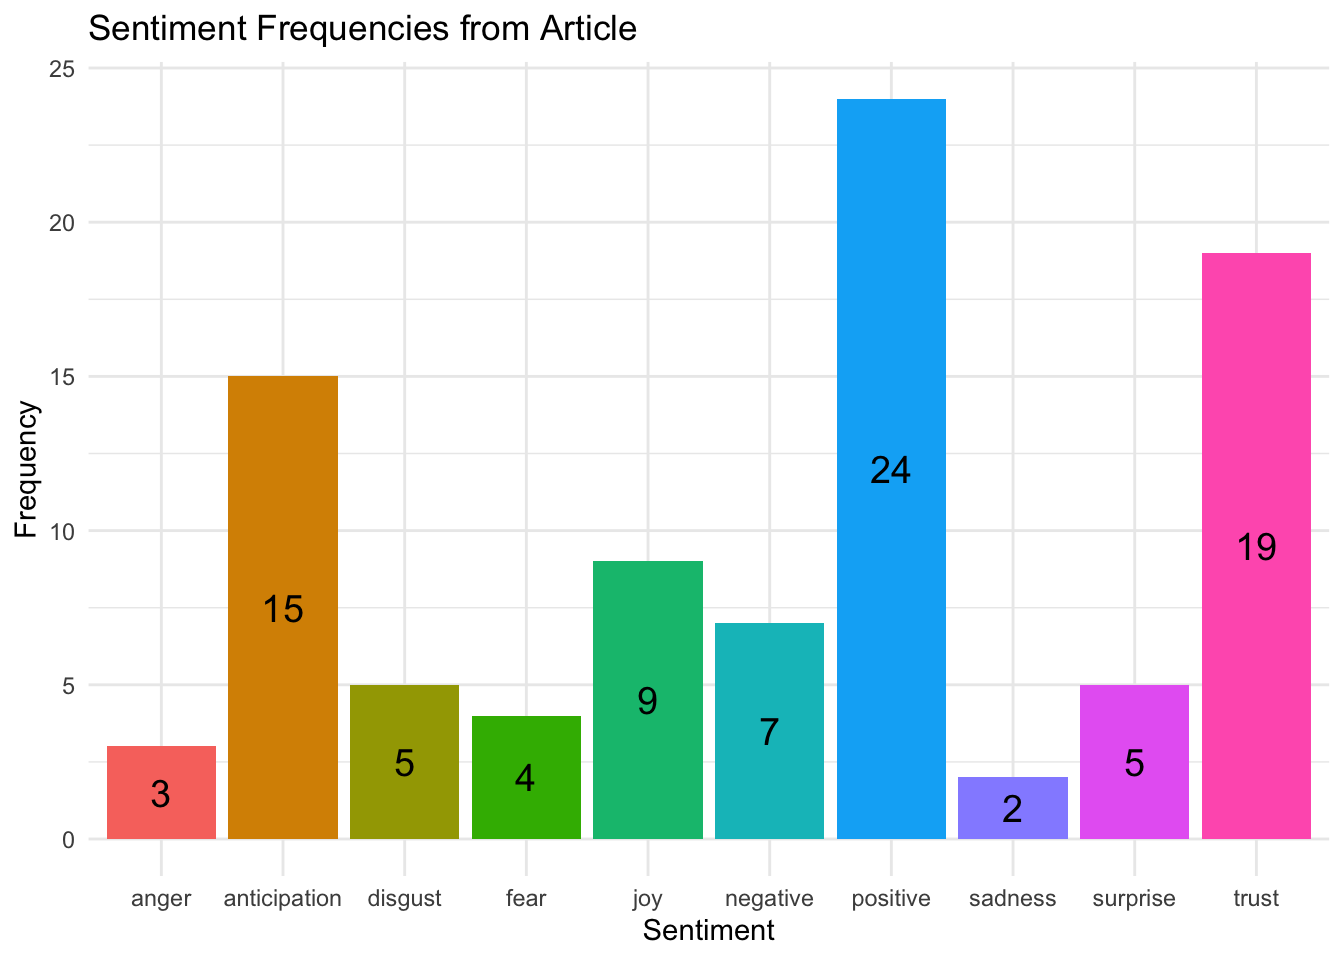
\includegraphics{Lab_sheet3_files/figure-latex/unnamed-chunk-17-1.pdf}

\begin{Shaded}
\begin{Highlighting}[]
\NormalTok{ptype }\OtherTok{\textless{}{-}} \FunctionTok{rep}\NormalTok{(}\StringTok{"other"}\NormalTok{,}\FunctionTok{length}\NormalTok{(}\AttributeTok{x=}\NormalTok{x))}
\NormalTok{ptype[x}\SpecialCharTok{\textless{}=}\NormalTok{y] }\OtherTok{\textless{}{-}} \StringTok{"x\textless{}=y"}
\NormalTok{ptype[(x}\SpecialCharTok{\textless{}=}\DecValTok{15} \SpecialCharTok{\&}\NormalTok{ x}\SpecialCharTok{\textgreater{}=}\DecValTok{5}\NormalTok{) }\SpecialCharTok{\&}\NormalTok{ (y}\SpecialCharTok{\textless{}=}\DecValTok{15} \SpecialCharTok{\&}\NormalTok{ y}\SpecialCharTok{\textgreater{}=}\DecValTok{5}\NormalTok{)] }\OtherTok{\textless{}{-}} \StringTok{"favourable"}
\NormalTok{ptype[y}\SpecialCharTok{==}\FunctionTok{max}\NormalTok{(y)]}\OtherTok{\textless{}{-}}\StringTok{"peak"}
\NormalTok{ptype }\OtherTok{\textless{}{-}} \FunctionTok{factor}\NormalTok{(}\AttributeTok{x=}\NormalTok{ptype)}
\NormalTok{ptype}
\end{Highlighting}
\end{Shaded}

\begin{verbatim}
##  [1] x<=y       other      other      other      other      x<=y       favourable
##  [8] favourable favourable favourable favourable other      other      other     
## [15] favourable x<=y       x<=y       peak       x<=y       x<=y      
## Levels: favourable other peak x<=y
\end{verbatim}

\begin{Shaded}
\begin{Highlighting}[]
\FunctionTok{qplot}\NormalTok{(x,y,}\AttributeTok{color=}\NormalTok{ptype,}\AttributeTok{shape=}\NormalTok{ptype)}
\end{Highlighting}
\end{Shaded}

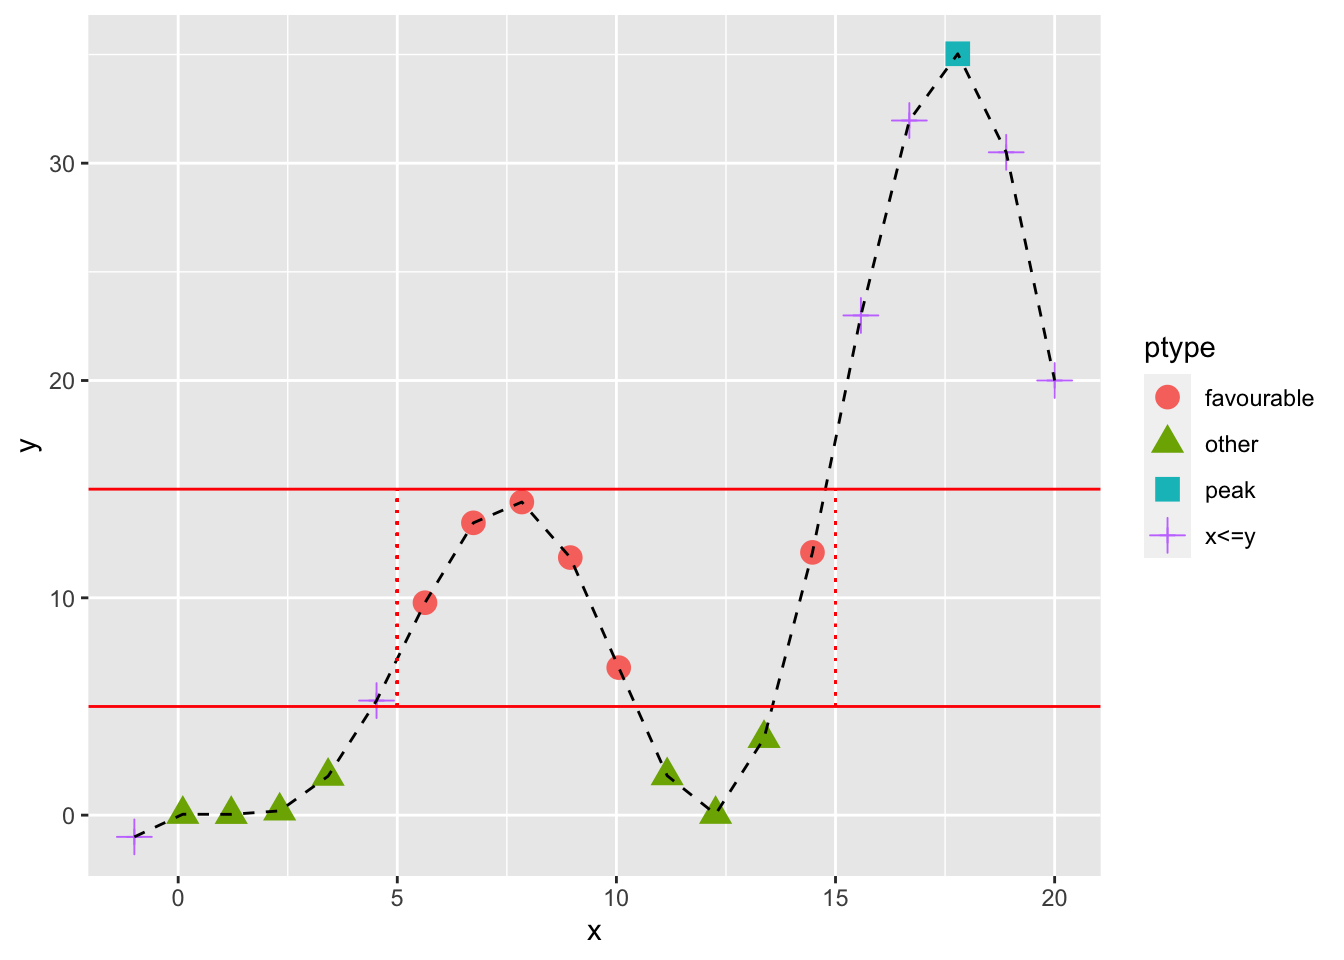
\includegraphics{Lab_sheet3_files/figure-latex/unnamed-chunk-18-1.pdf}

\begin{Shaded}
\begin{Highlighting}[]
\FunctionTok{qplot}\NormalTok{(x,y,}\AttributeTok{color=}\NormalTok{ptype,}\AttributeTok{shape=}\NormalTok{ptype) }\SpecialCharTok{+} \FunctionTok{geom\_point}\NormalTok{(}\AttributeTok{size=}\DecValTok{4}\NormalTok{) }\SpecialCharTok{+}
\FunctionTok{geom\_line}\NormalTok{(}\AttributeTok{mapping=}\FunctionTok{aes}\NormalTok{(}\AttributeTok{group=}\DecValTok{1}\NormalTok{),}\AttributeTok{color=}\StringTok{"black"}\NormalTok{,}\AttributeTok{lty=}\DecValTok{2}\NormalTok{) }\SpecialCharTok{+}
\FunctionTok{geom\_hline}\NormalTok{(}\AttributeTok{mapping=}\FunctionTok{aes}\NormalTok{(}\AttributeTok{yintercept=}\FunctionTok{c}\NormalTok{(}\DecValTok{5}\NormalTok{,}\DecValTok{15}\NormalTok{)),}\AttributeTok{color=}\StringTok{"red"}\NormalTok{)}\SpecialCharTok{+}
\FunctionTok{geom\_segment}\NormalTok{(}\AttributeTok{mapping=}\FunctionTok{aes}\NormalTok{(}\AttributeTok{x=}\DecValTok{5}\NormalTok{,}\AttributeTok{y=}\DecValTok{5}\NormalTok{,}\AttributeTok{xend=}\DecValTok{5}\NormalTok{,}\AttributeTok{yend=}\DecValTok{15}\NormalTok{),}\AttributeTok{color=}\StringTok{"red"}\NormalTok{,}\AttributeTok{lty=}\DecValTok{3}\NormalTok{)}\SpecialCharTok{+}
\FunctionTok{geom\_segment}\NormalTok{(}\AttributeTok{mapping=}\FunctionTok{aes}\NormalTok{(}\AttributeTok{x=}\DecValTok{15}\NormalTok{,}\AttributeTok{y=}\DecValTok{5}\NormalTok{,}\AttributeTok{xend=}\DecValTok{15}\NormalTok{,}\AttributeTok{yend=}\DecValTok{15}\NormalTok{),}\AttributeTok{color=}\StringTok{"red"}\NormalTok{,}\AttributeTok{lty=}\DecValTok{3}\NormalTok{)}
\end{Highlighting}
\end{Shaded}

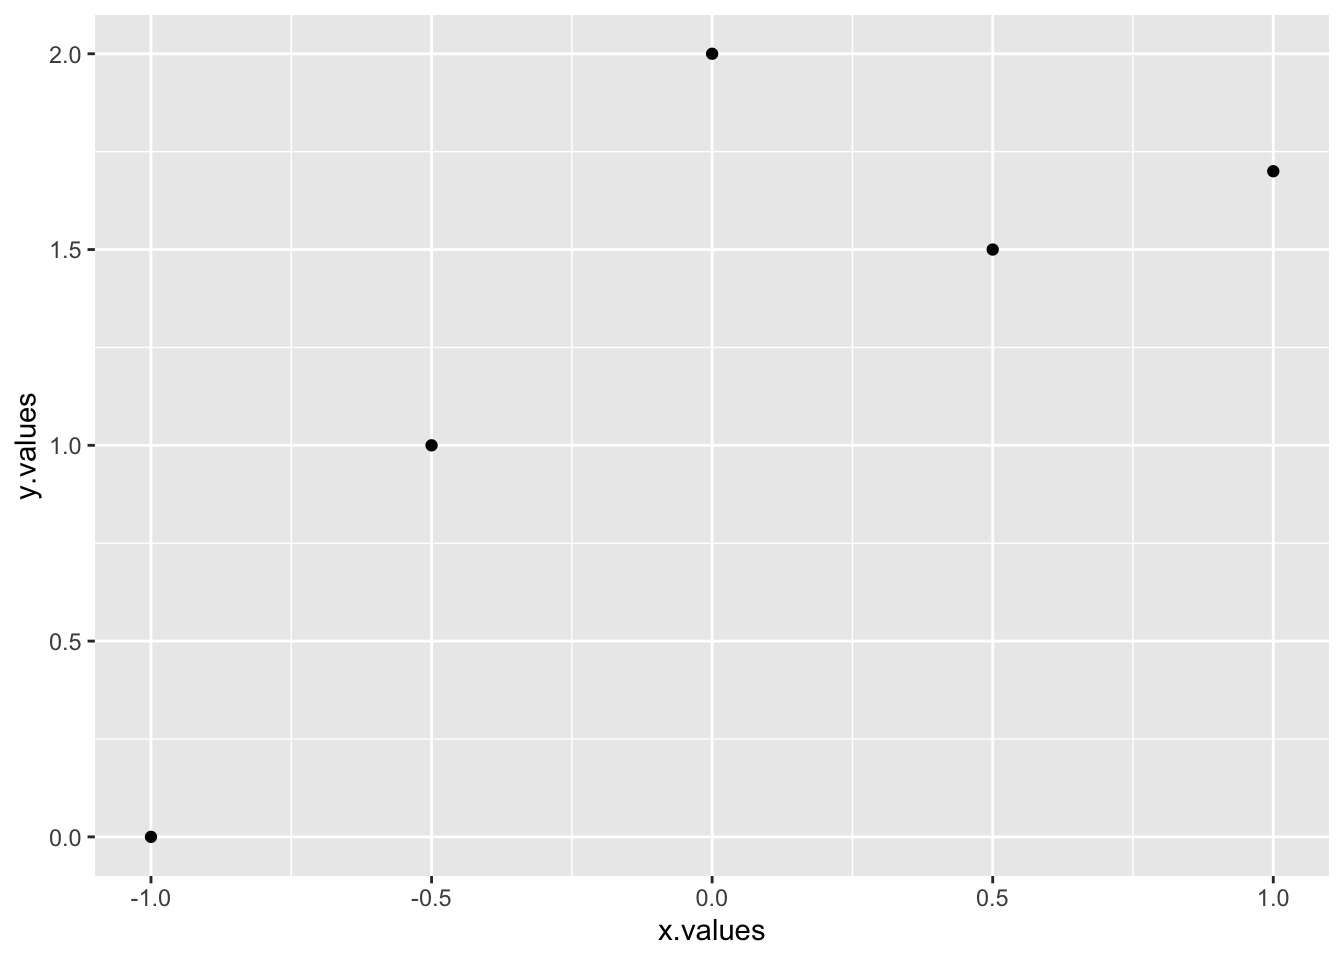
\includegraphics{Lab_sheet3_files/figure-latex/unnamed-chunk-19-1.pdf}

\begin{Shaded}
\begin{Highlighting}[]
\NormalTok{x1}\OtherTok{=}\FunctionTok{seq}\NormalTok{(}\AttributeTok{from=}\SpecialCharTok{{-}}\NormalTok{pi,}\AttributeTok{to=}\NormalTok{pi,}\AttributeTok{length.out =}\DecValTok{100}\NormalTok{)}
\NormalTok{y1 }\OtherTok{\textless{}{-}} \FunctionTok{sin}\NormalTok{(x1) }
\NormalTok{y2 }\OtherTok{\textless{}{-}} \FunctionTok{cos}\NormalTok{(x1)}
\NormalTok{mydata}\OtherTok{=}\FunctionTok{data.frame}\NormalTok{(}\AttributeTok{x=}\NormalTok{x1,}\AttributeTok{sin=}\NormalTok{y1,}\AttributeTok{cos=}\NormalTok{y2)}
\FunctionTok{ggplot}\NormalTok{(}\AttributeTok{data =}\NormalTok{ mydata)}\SpecialCharTok{+}
\FunctionTok{geom\_ribbon}\NormalTok{(}\FunctionTok{aes}\NormalTok{(}\AttributeTok{x=}\NormalTok{x, }\AttributeTok{ymax=}\NormalTok{cos, }\AttributeTok{ymin=}\NormalTok{sin), }\AttributeTok{fill=}\StringTok{"gray"}\NormalTok{)}\SpecialCharTok{+}
\FunctionTok{geom\_line}\NormalTok{(}\FunctionTok{aes}\NormalTok{(}\AttributeTok{x=}\NormalTok{x,}\AttributeTok{y =}\NormalTok{ sin), }\AttributeTok{colour =} \StringTok{\textquotesingle{}red\textquotesingle{}}\NormalTok{) }\SpecialCharTok{+}
\FunctionTok{geom\_line}\NormalTok{(}\FunctionTok{aes}\NormalTok{(}\AttributeTok{x=}\NormalTok{x,}\AttributeTok{y =}\NormalTok{ cos), }\AttributeTok{colour =} \StringTok{\textquotesingle{}blue\textquotesingle{}}\NormalTok{)}
\end{Highlighting}
\end{Shaded}

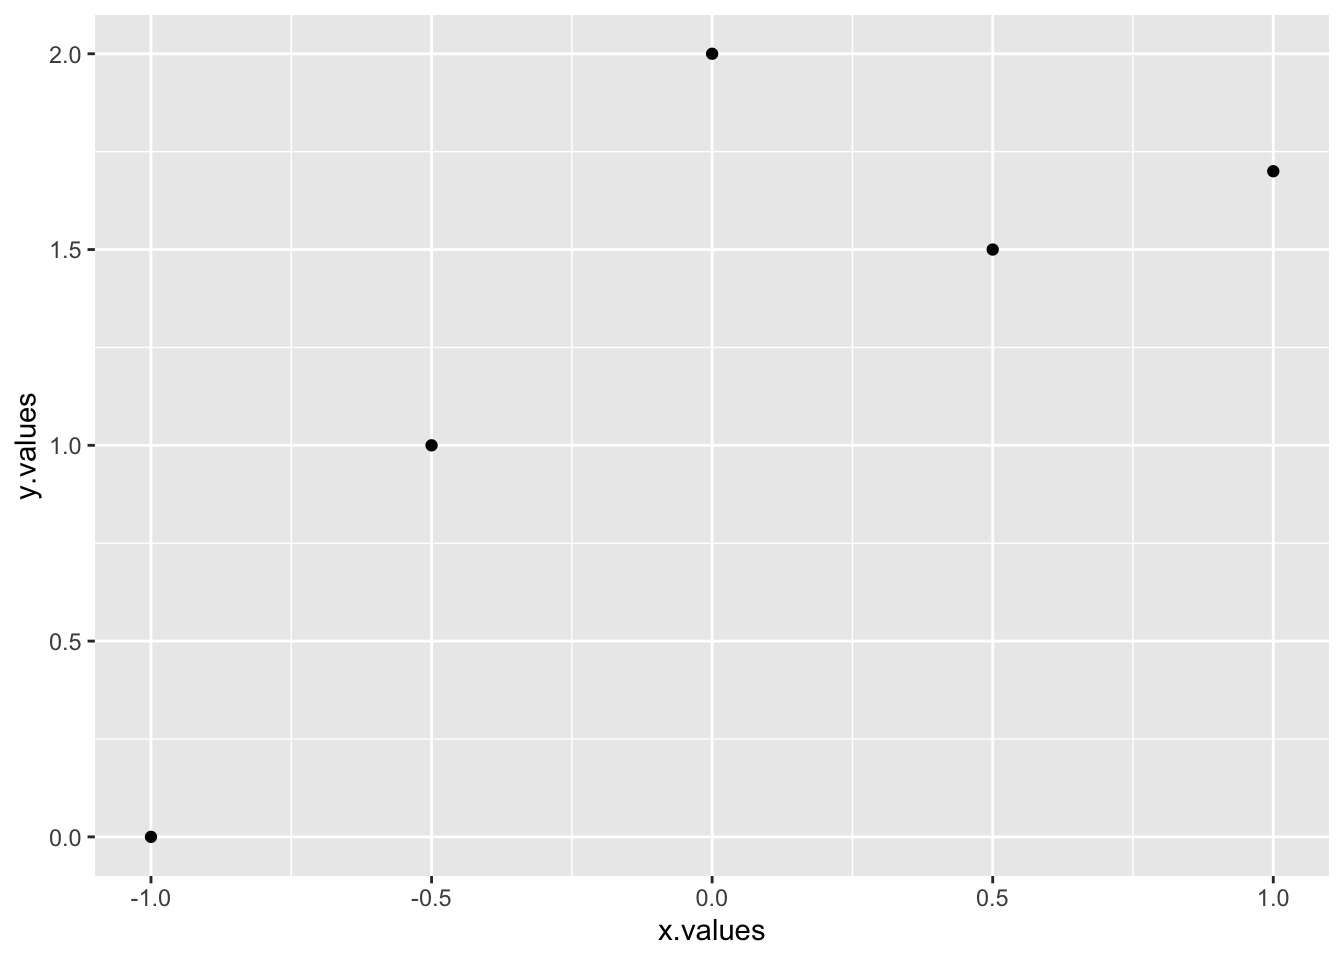
\includegraphics{Lab_sheet3_files/figure-latex/unnamed-chunk-20-1.pdf}

\end{document}
